\title{3D BEM: Shape and Tension}
\author{
        Joseph M. Barakat
}
\date{\today}
%the percentage makes comments
%this is the preamble where all the packages are loaded. I would always have these packages.
\documentclass[12pt]{article}
\usepackage[english]{babel}
\usepackage{graphicx}%this allows you to add figures
\usepackage{float}
\usepackage{amsmath}%this lets you write math
\usepackage{mathtools}
\usepackage{amssymb}%this lets you write math symbols
\usepackage{mathrsfs}
\numberwithin{equation}{section}
\usepackage{caption}%this lets you caption figure
\usepackage{wrapfig}
\usepackage{setspace}%this lets you control line spacing
\usepackage{siunitx}%this lets you make SI units
\usepackage[margin=1in]{geometry}
\usepackage[version=3]{mhchem}
\usepackage{csquotes}
\usepackage{cancel}
\usepackage{esint}
\usepackage{courier}
\usepackage{bm,upgreek}
\usepackage{braket}
%\usepackage{wasysym}
%\usepackage{breqn}
\usepackage{appendix}
\usepackage{stmaryrd}
\usepackage{hyperref}
\usepackage[final]{pdfpages}
\usepackage{bbm}
%\usepackage{calligra}
%\usepackage[T1]{fontenc}
\usepackage{perpage}
\MakePerPage{footnote}

% Insert MATLAB and Mathematica  code into document
\usepackage{listings}
\lstloadlanguages{[5.2]Mathematica}
\usepackage{color} %red, green, blue, yellow, cyan, magenta, black, white
\definecolor{mygreen}{RGB}{28,172,0} % color values Red, Green, Blue
\definecolor{mylilas}{RGB}{170,55,241}

\DeclareMathOperator{\tr}{tr}
\DeclareMathOperator{\sech}{sech}
%
%\DeclareMathAlphabet{\mathcalligra}{T1}{calligra}{m}{n}
%\DeclareFontShape{T1}{calligra}{m}{n}{<->s*[1.7]callig15}{}

\begin{document}
\maketitle

\allowdisplaybreaks[1]

\renewcommand*{\thefootnote}{\fnsymbol{footnote}}

% Insert MATLAB script into text
\lstset{language=MATLAB,%
    %basicstyle=\color{red},
    breaklines=true,%
    morekeywords={matlab2tikz},
    keywordstyle=\color{blue},%
    morekeywords=[2]{1}, keywordstyle=[2]{\color{black}},
    identifierstyle=\color{black},%
    stringstyle=\color{mylilas},
    commentstyle=\color{mygreen},%
    showstringspaces=false,%without this there will be a symbol in the places where there is a space
    numbers=left,%
    numberstyle={\tiny \color{black}},% size of the numbers
    numbersep=9pt, % this defines how far the numbers are from the text
    emph=[1]{for,end,break},emphstyle=[1]\color{red}, %some words to emphasise
    %emph=[2]{word1,word2}, emphstyle=[2]{style},    
}

% To insert MATLAB script, type
%	\texttt{\lstinputlisting{[...].m}}

% To insert figure, type
%	\begin{figure}[h]
%	\begin{center}
%		\includegraphics[width=.45\textwidth]{[...].jpg}
%	\caption{...}
%	\label{fig:?}
%	\end{center}
%	\end{figure}

\pagebreak
\begin{figure}[h]
\begin{center}
	Ca = 0.03
	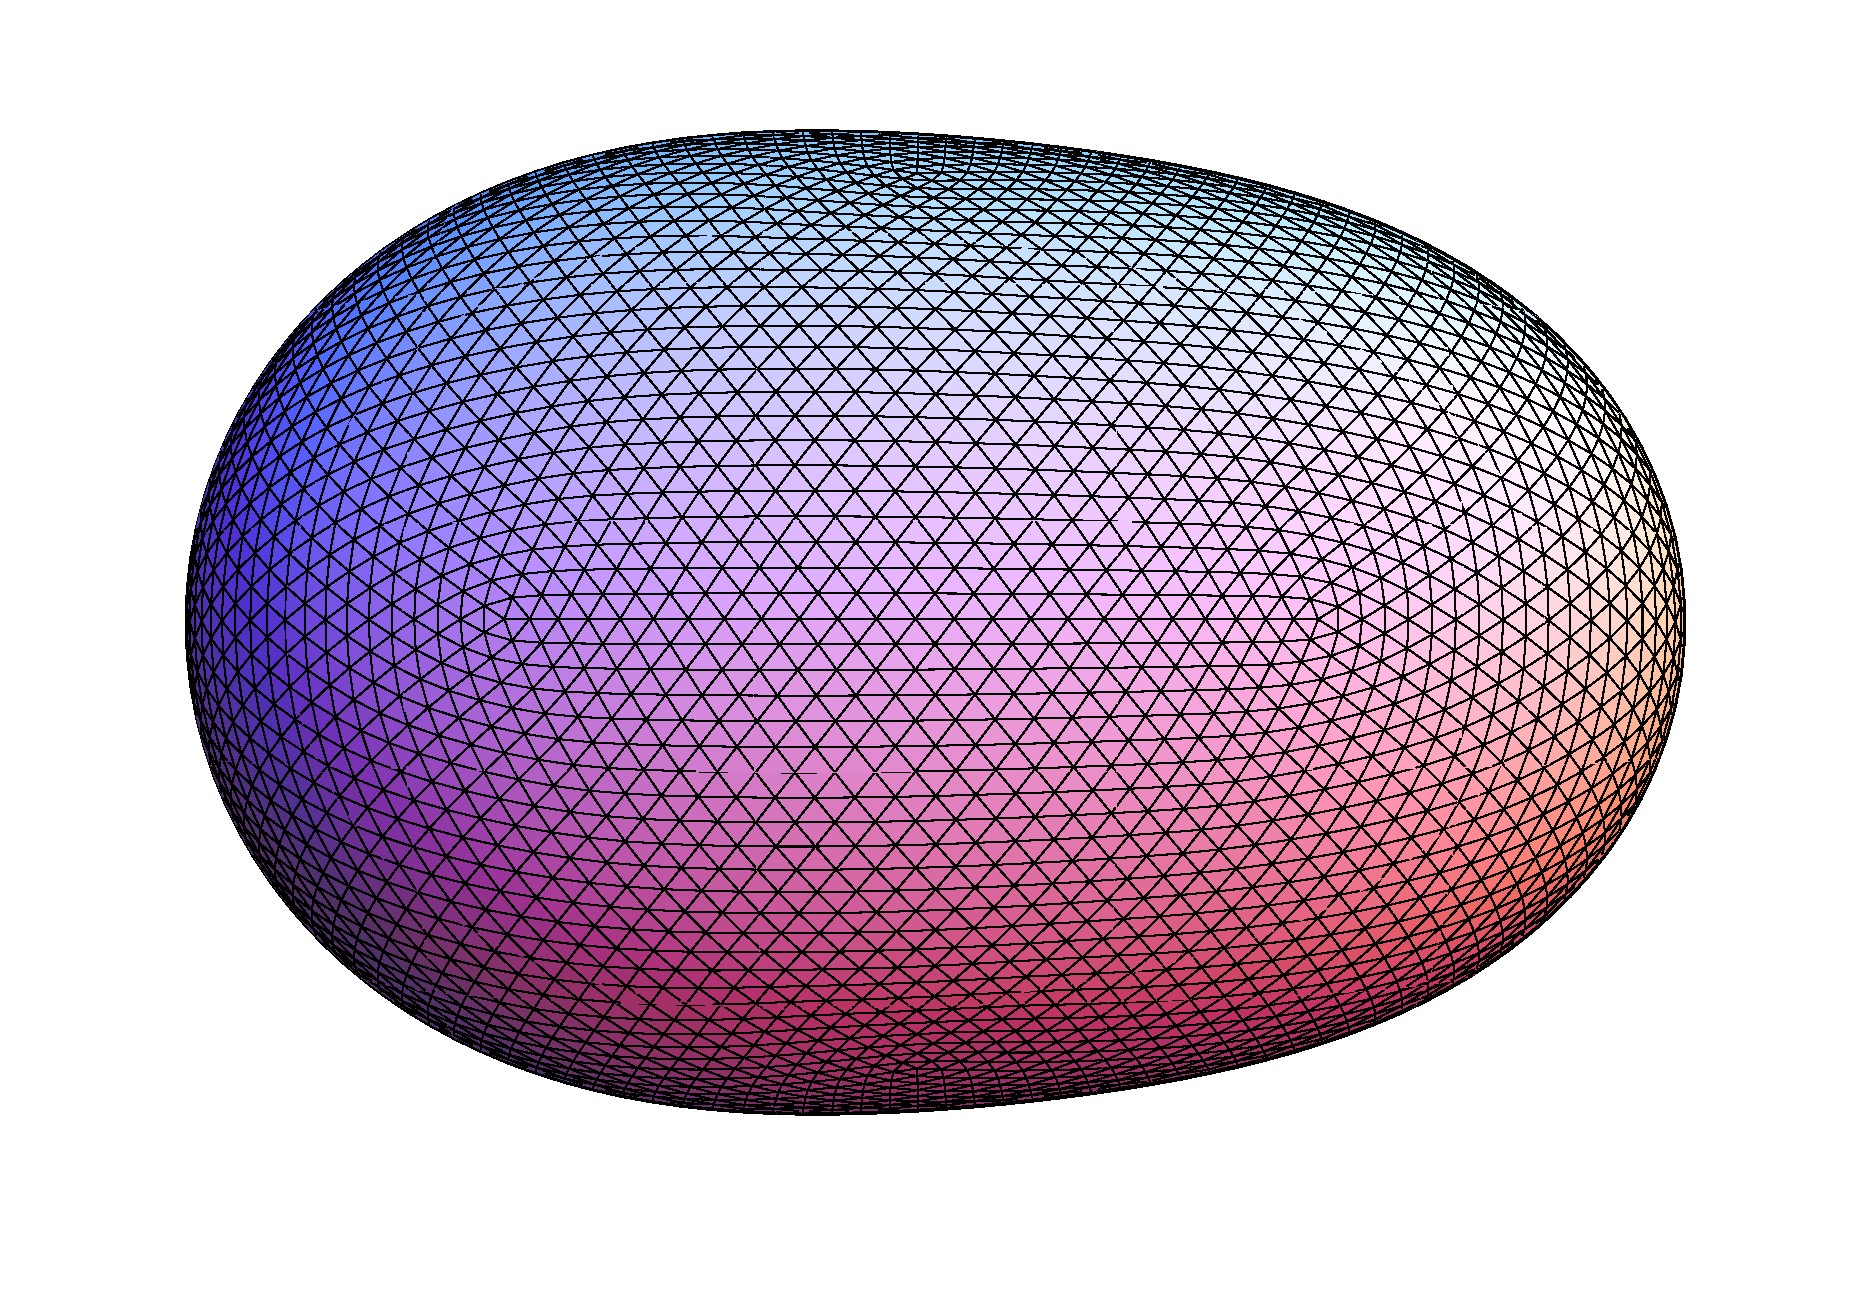
\includegraphics[width=0.4\textwidth]{shape/shape_vred95_conf90_v1eb20}
	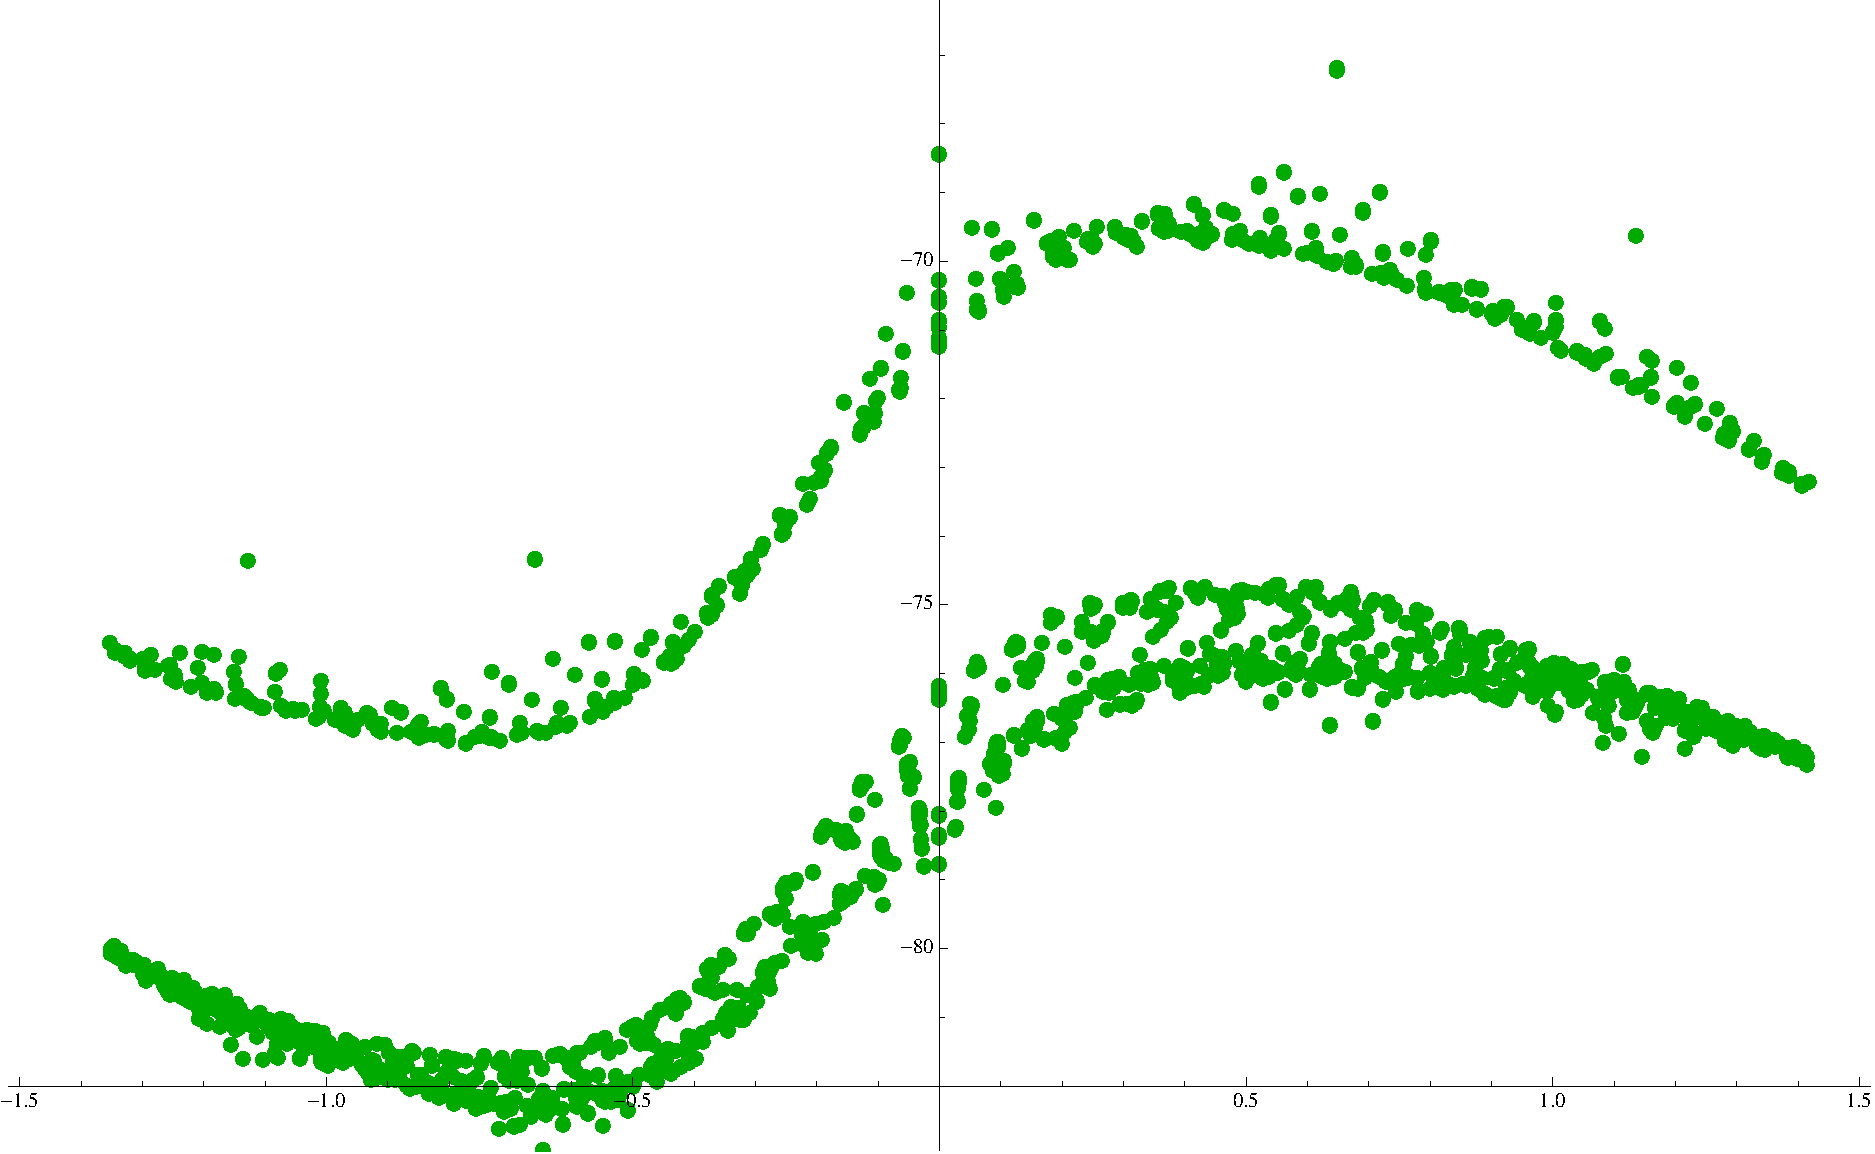
\includegraphics[width=0.4\textwidth]{tension/tension_vred95_conf90_v1eb20}
	\\
	Ca = 0.06
	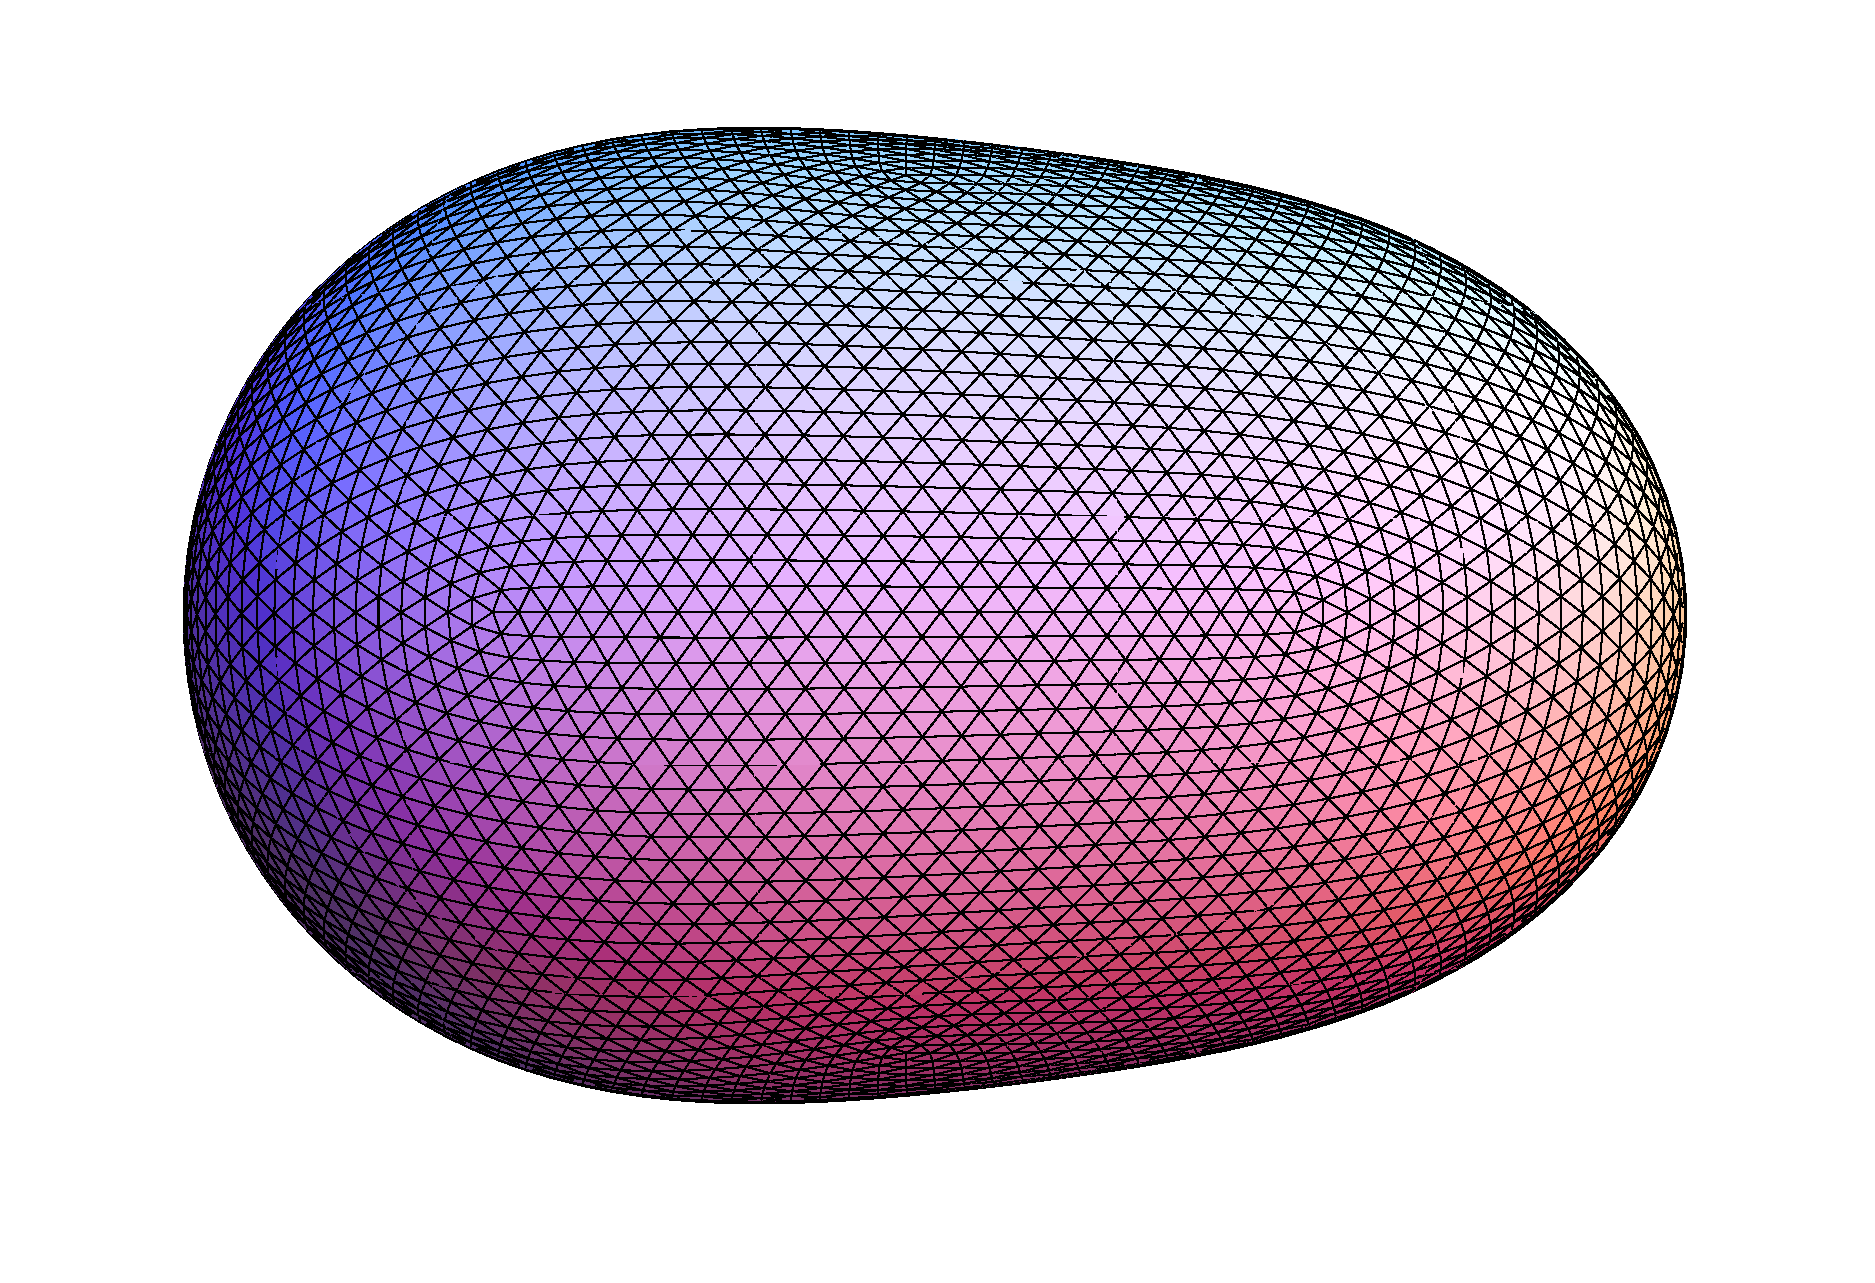
\includegraphics[width=0.4\textwidth]{shape/shape_vred95_conf90_v1eb10}
	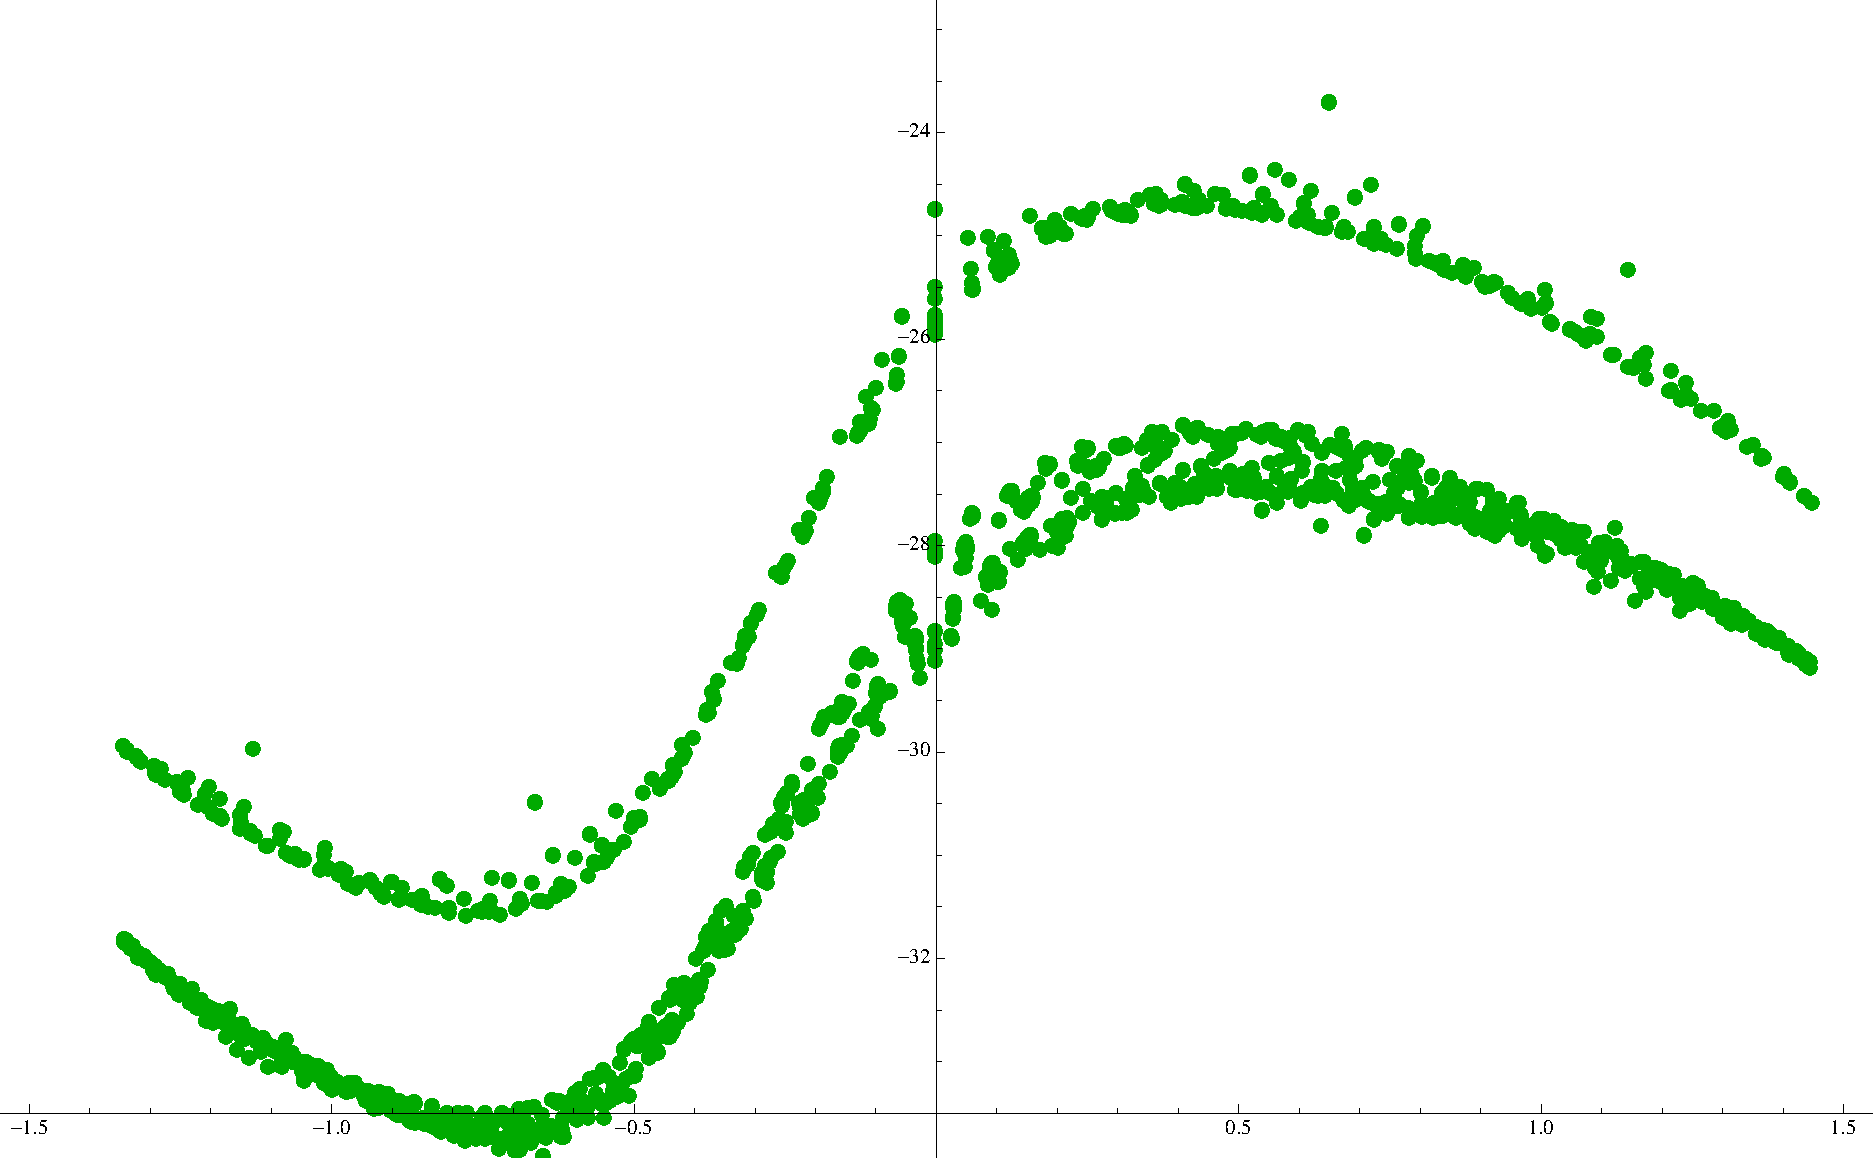
\includegraphics[width=0.4\textwidth]{tension/tension_vred95_conf90_v1eb10}
	\\
	Ca = 0.31
	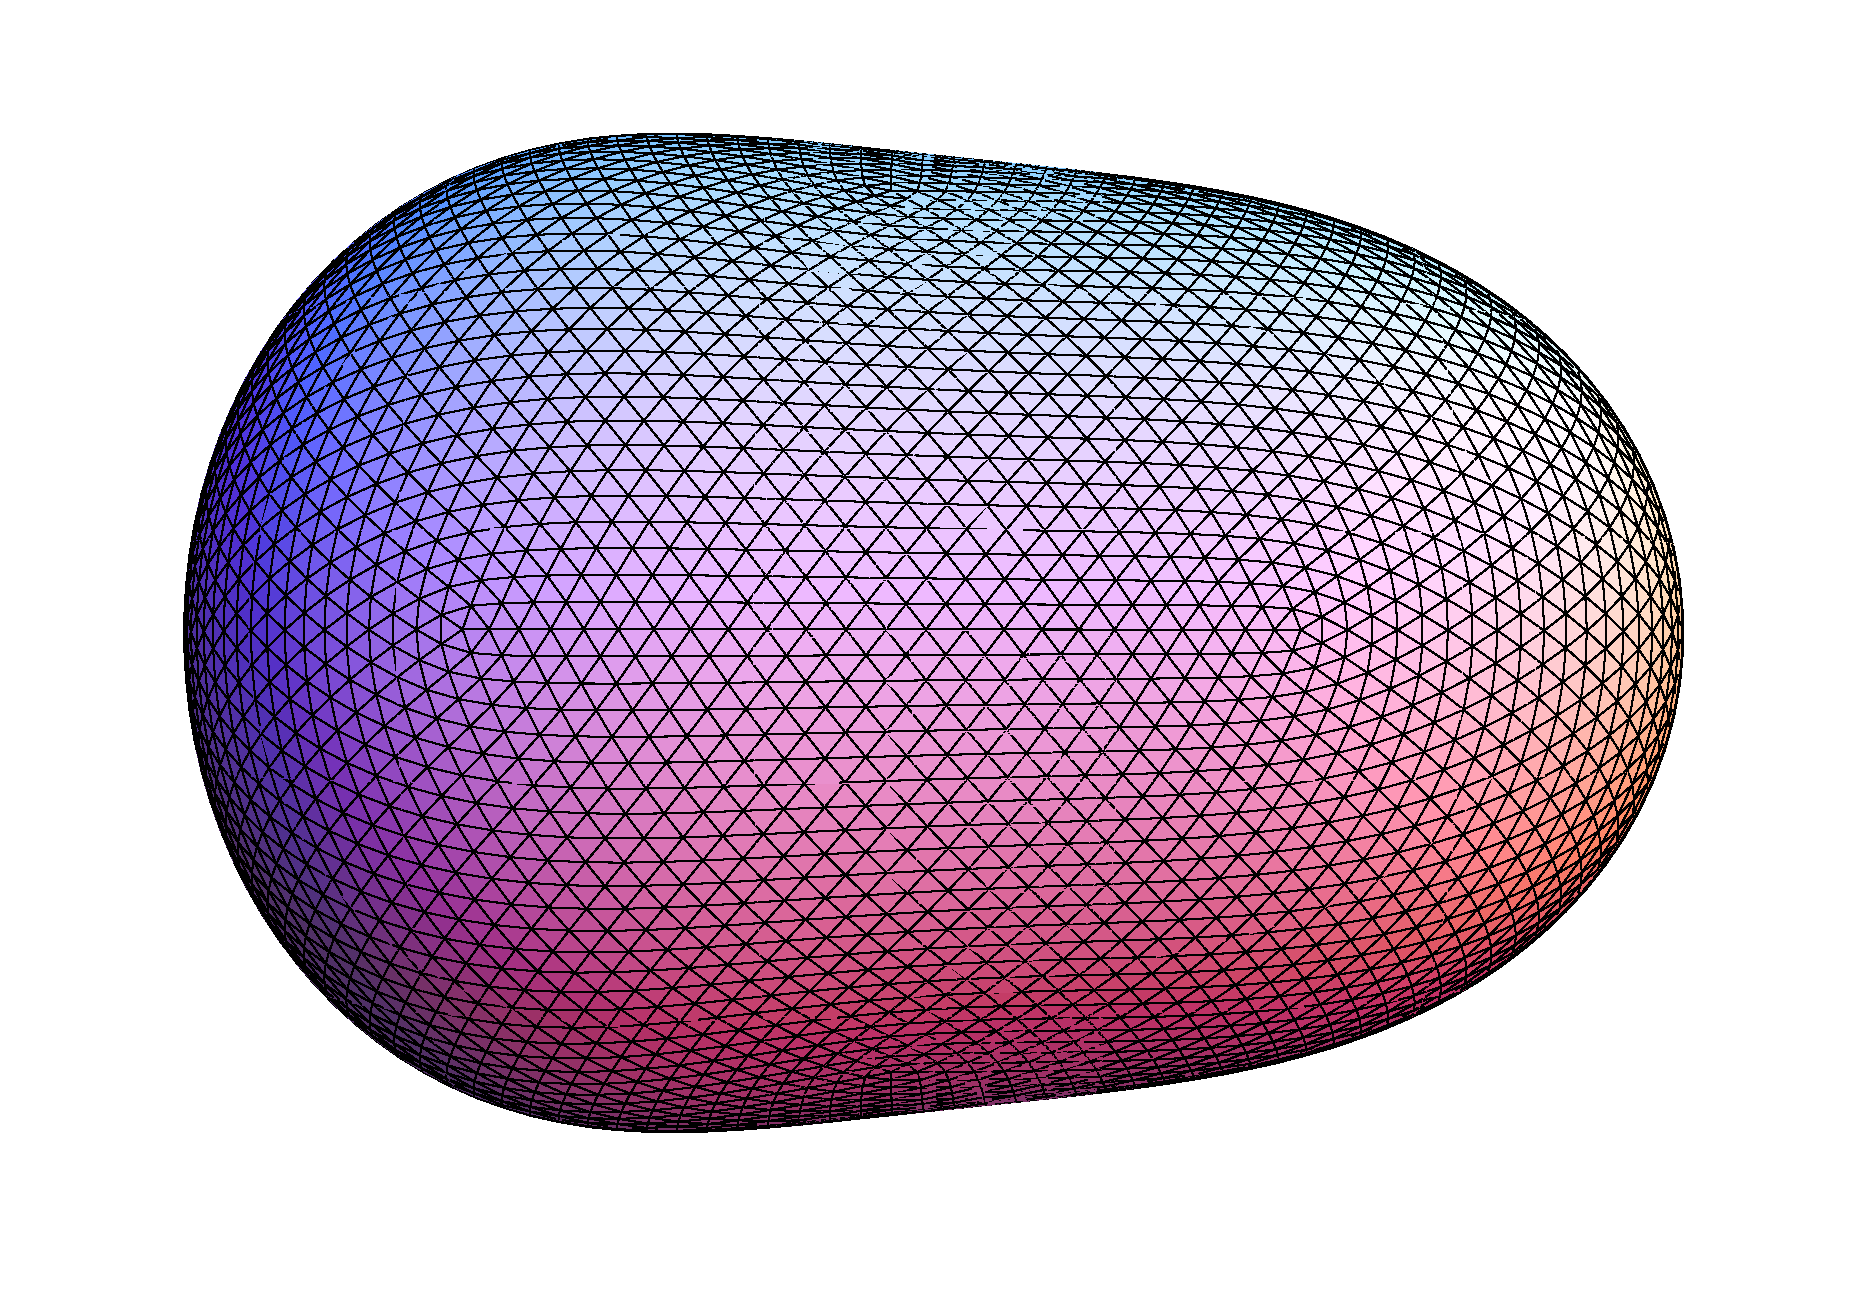
\includegraphics[width=0.4\textwidth]{shape/shape_vred95_conf90_v1eb2}
	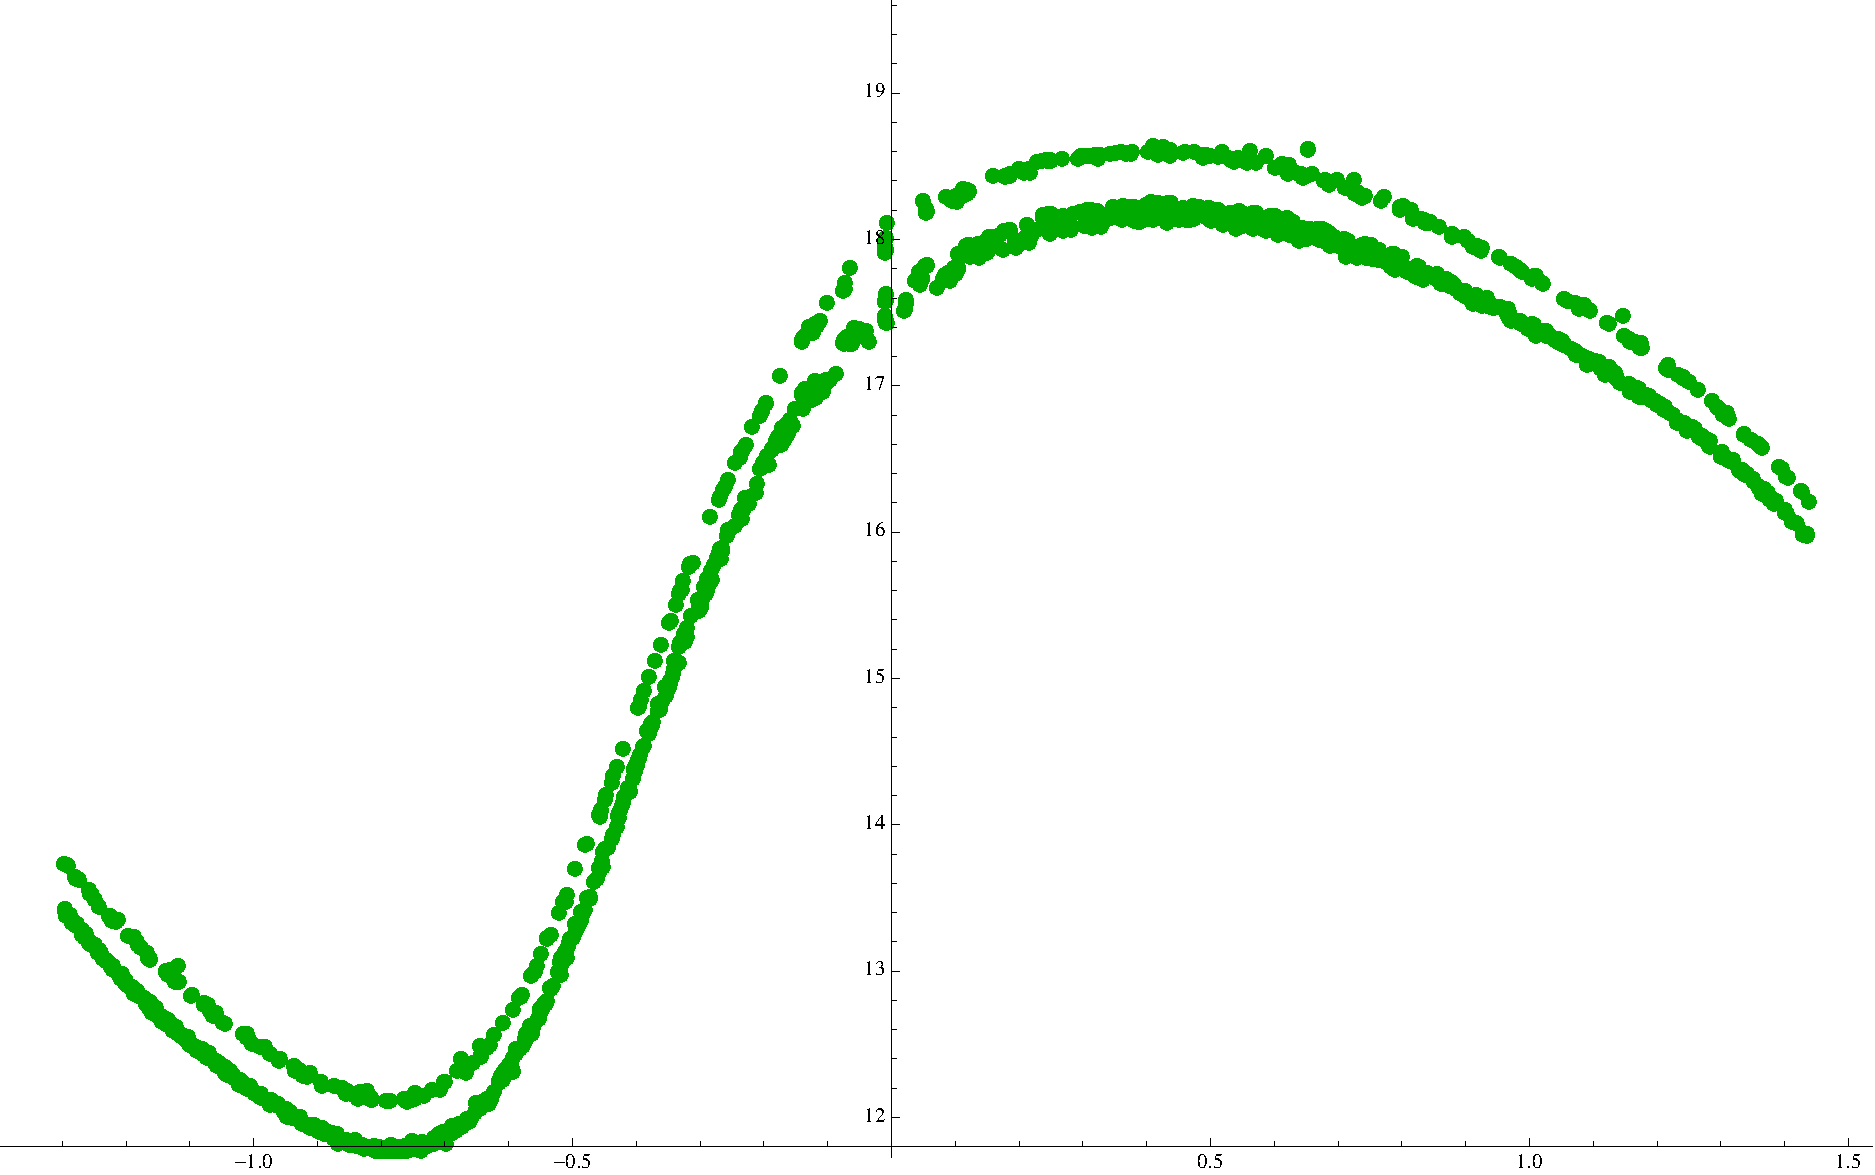
\includegraphics[width=0.4\textwidth]{tension/tension_vred95_conf90_v1eb2}
	\\
	Ca = 1.25 
	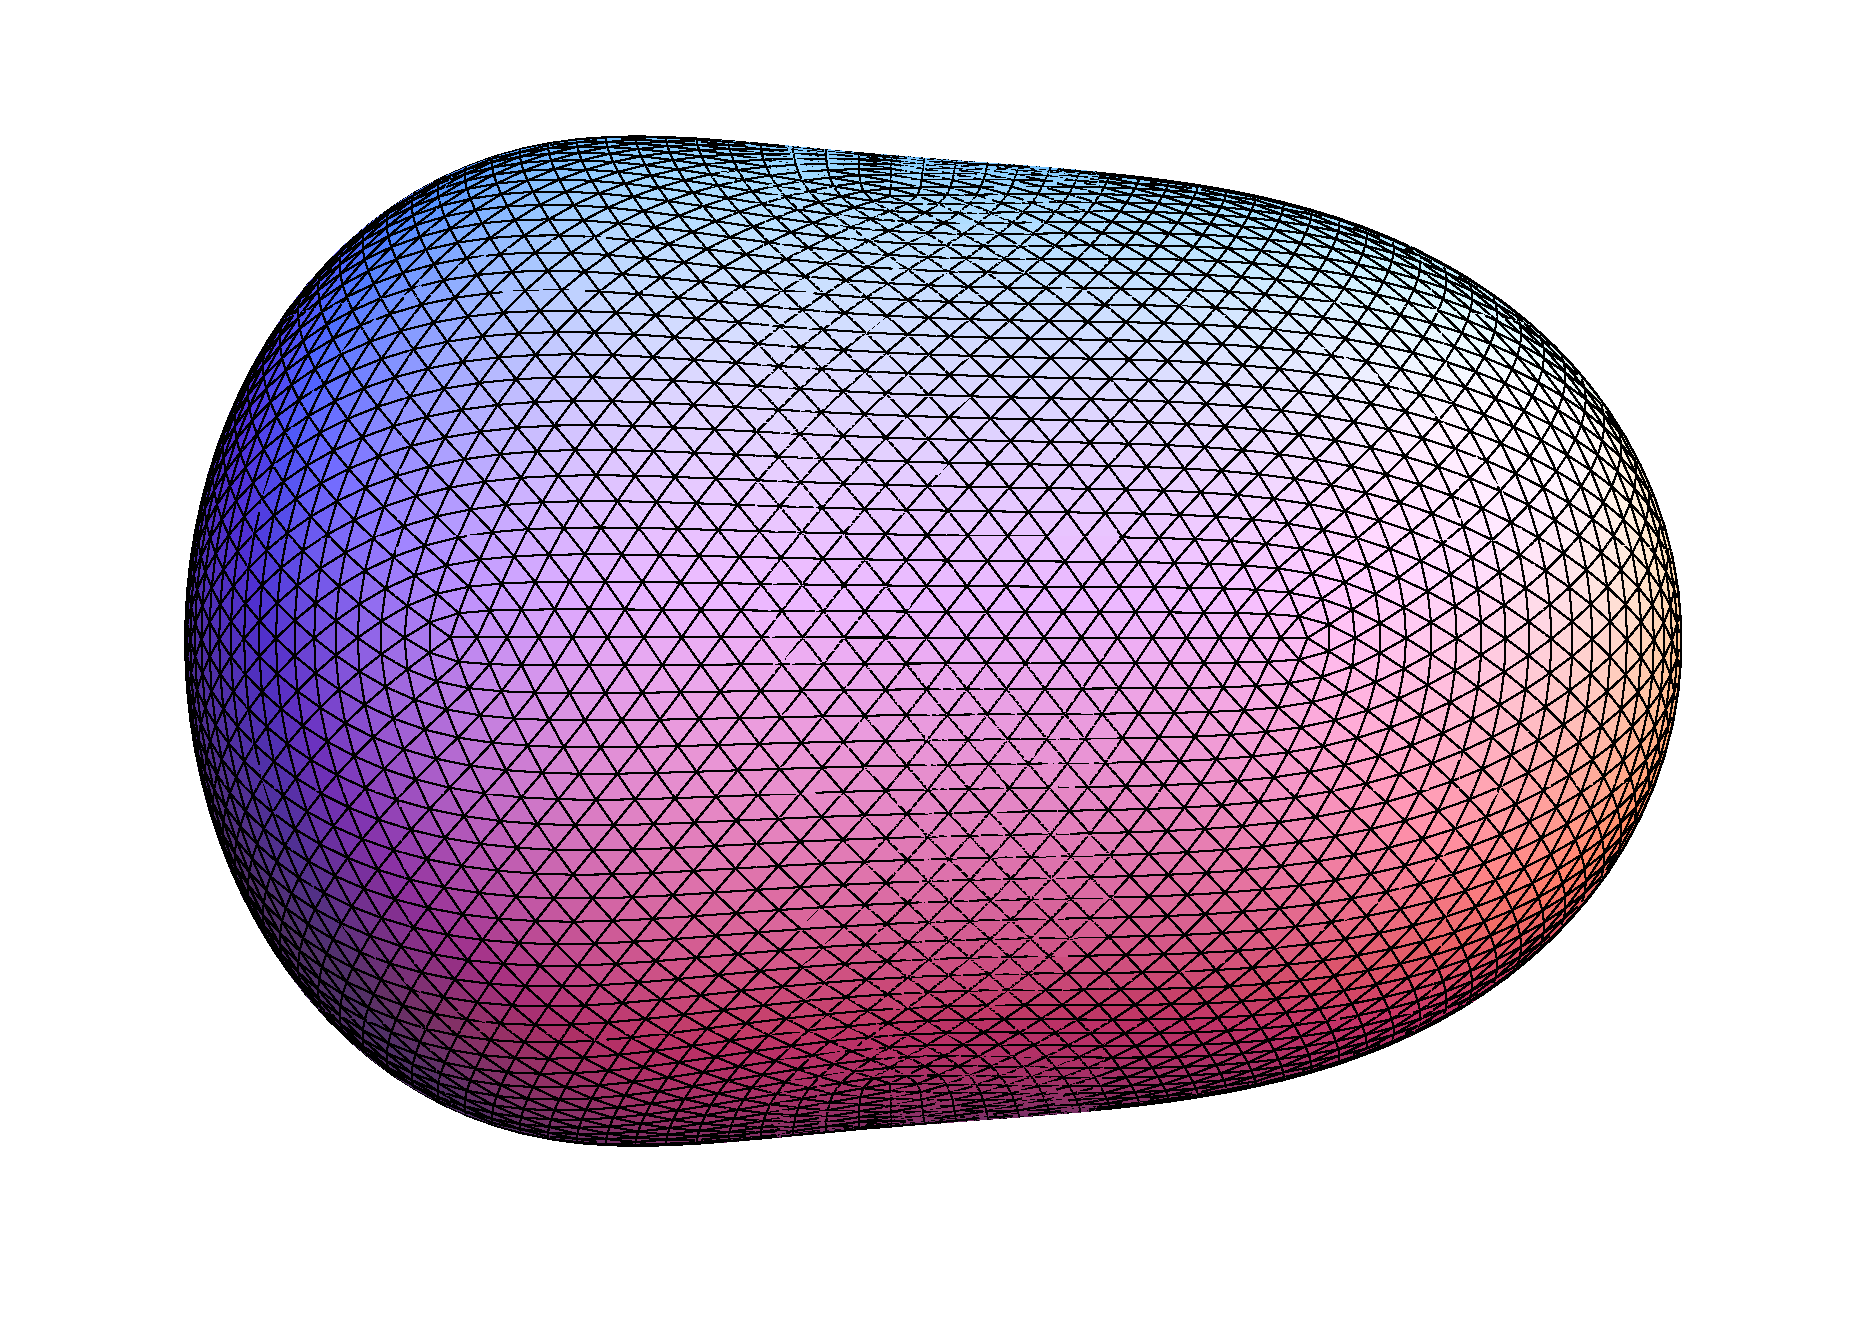
\includegraphics[width=0.4\textwidth]{shape/shape_vred95_conf90_v1eb05}
	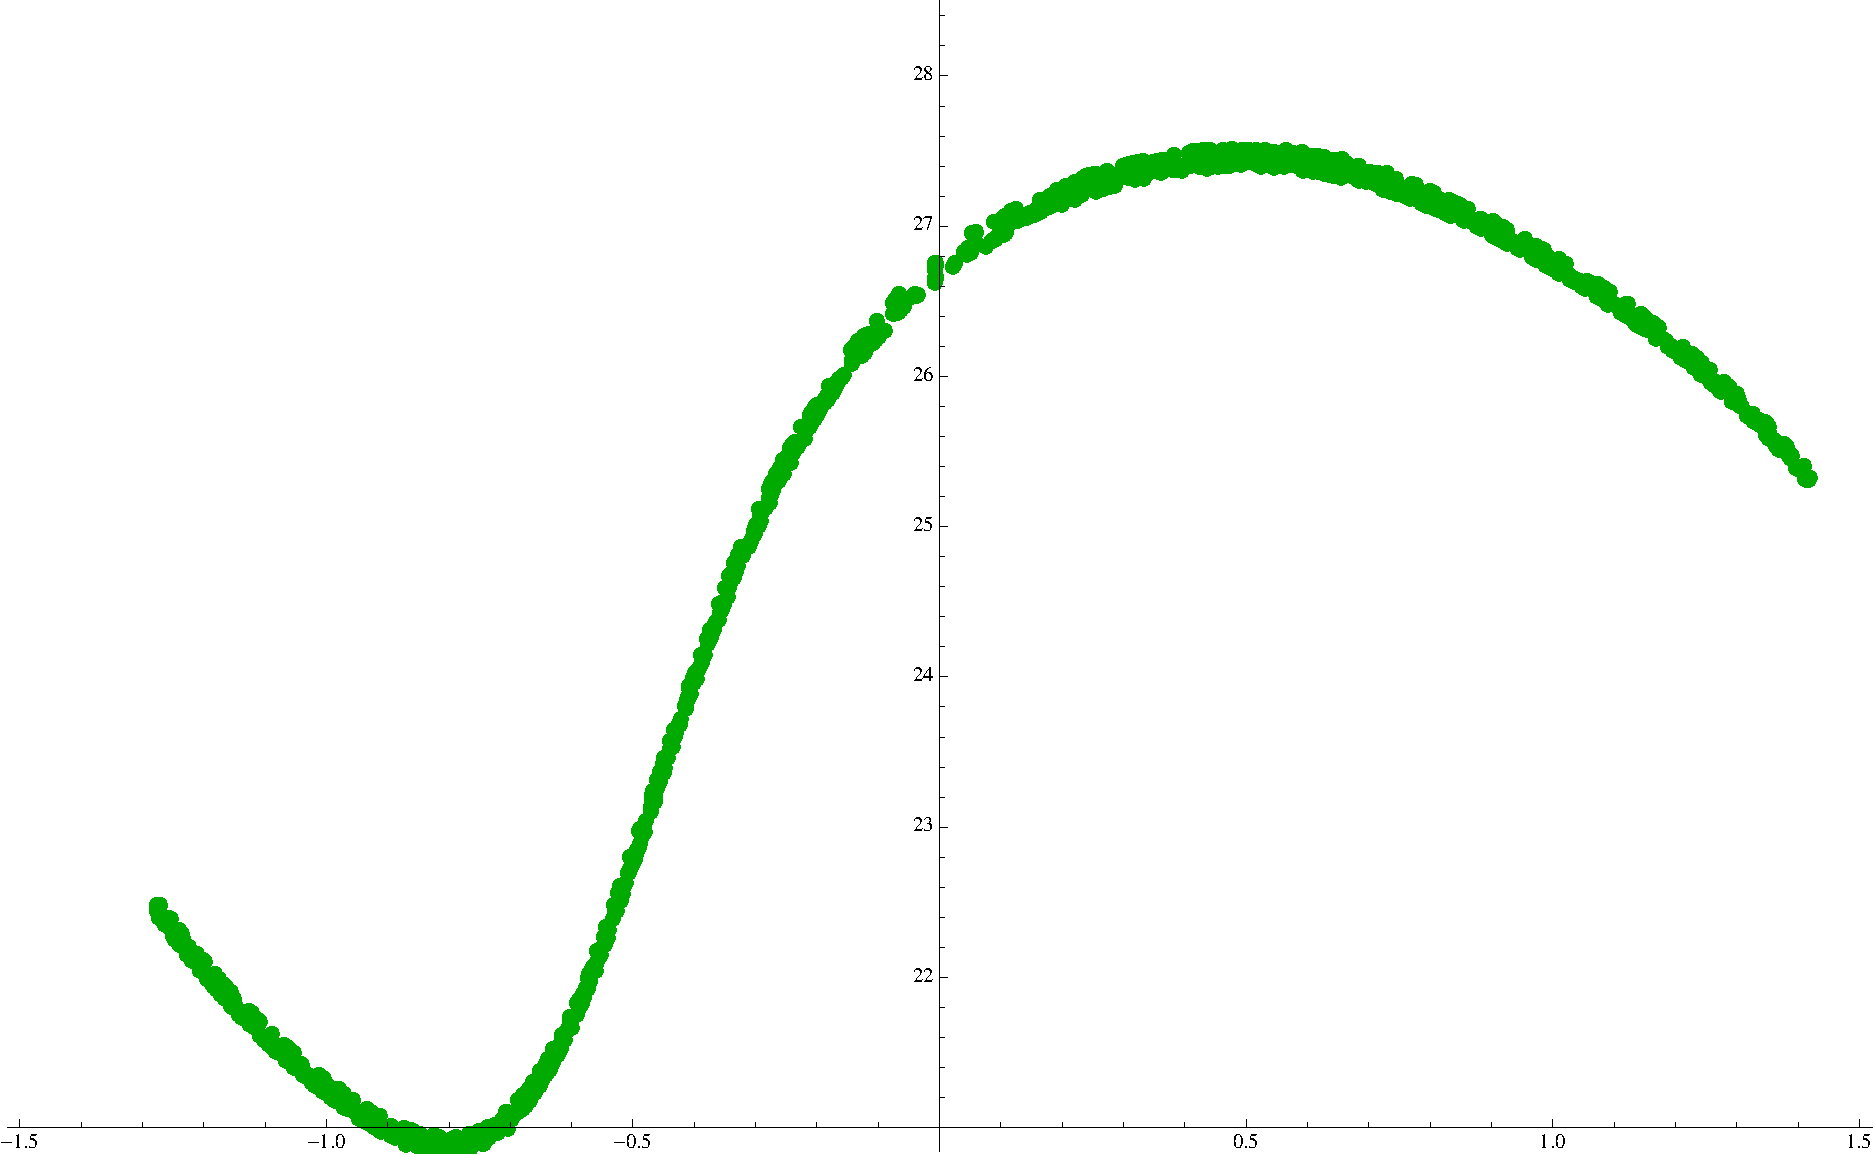
\includegraphics[width=0.4\textwidth]{tension/tension_vred95_conf90_v1eb05}
\caption{$\nu = 0.95$, conf = 0.90}
%\label{default}
\end{center}
\end{figure}

\pagebreak
\begin{figure}[h]
\begin{center}
	Ca = 0.03
	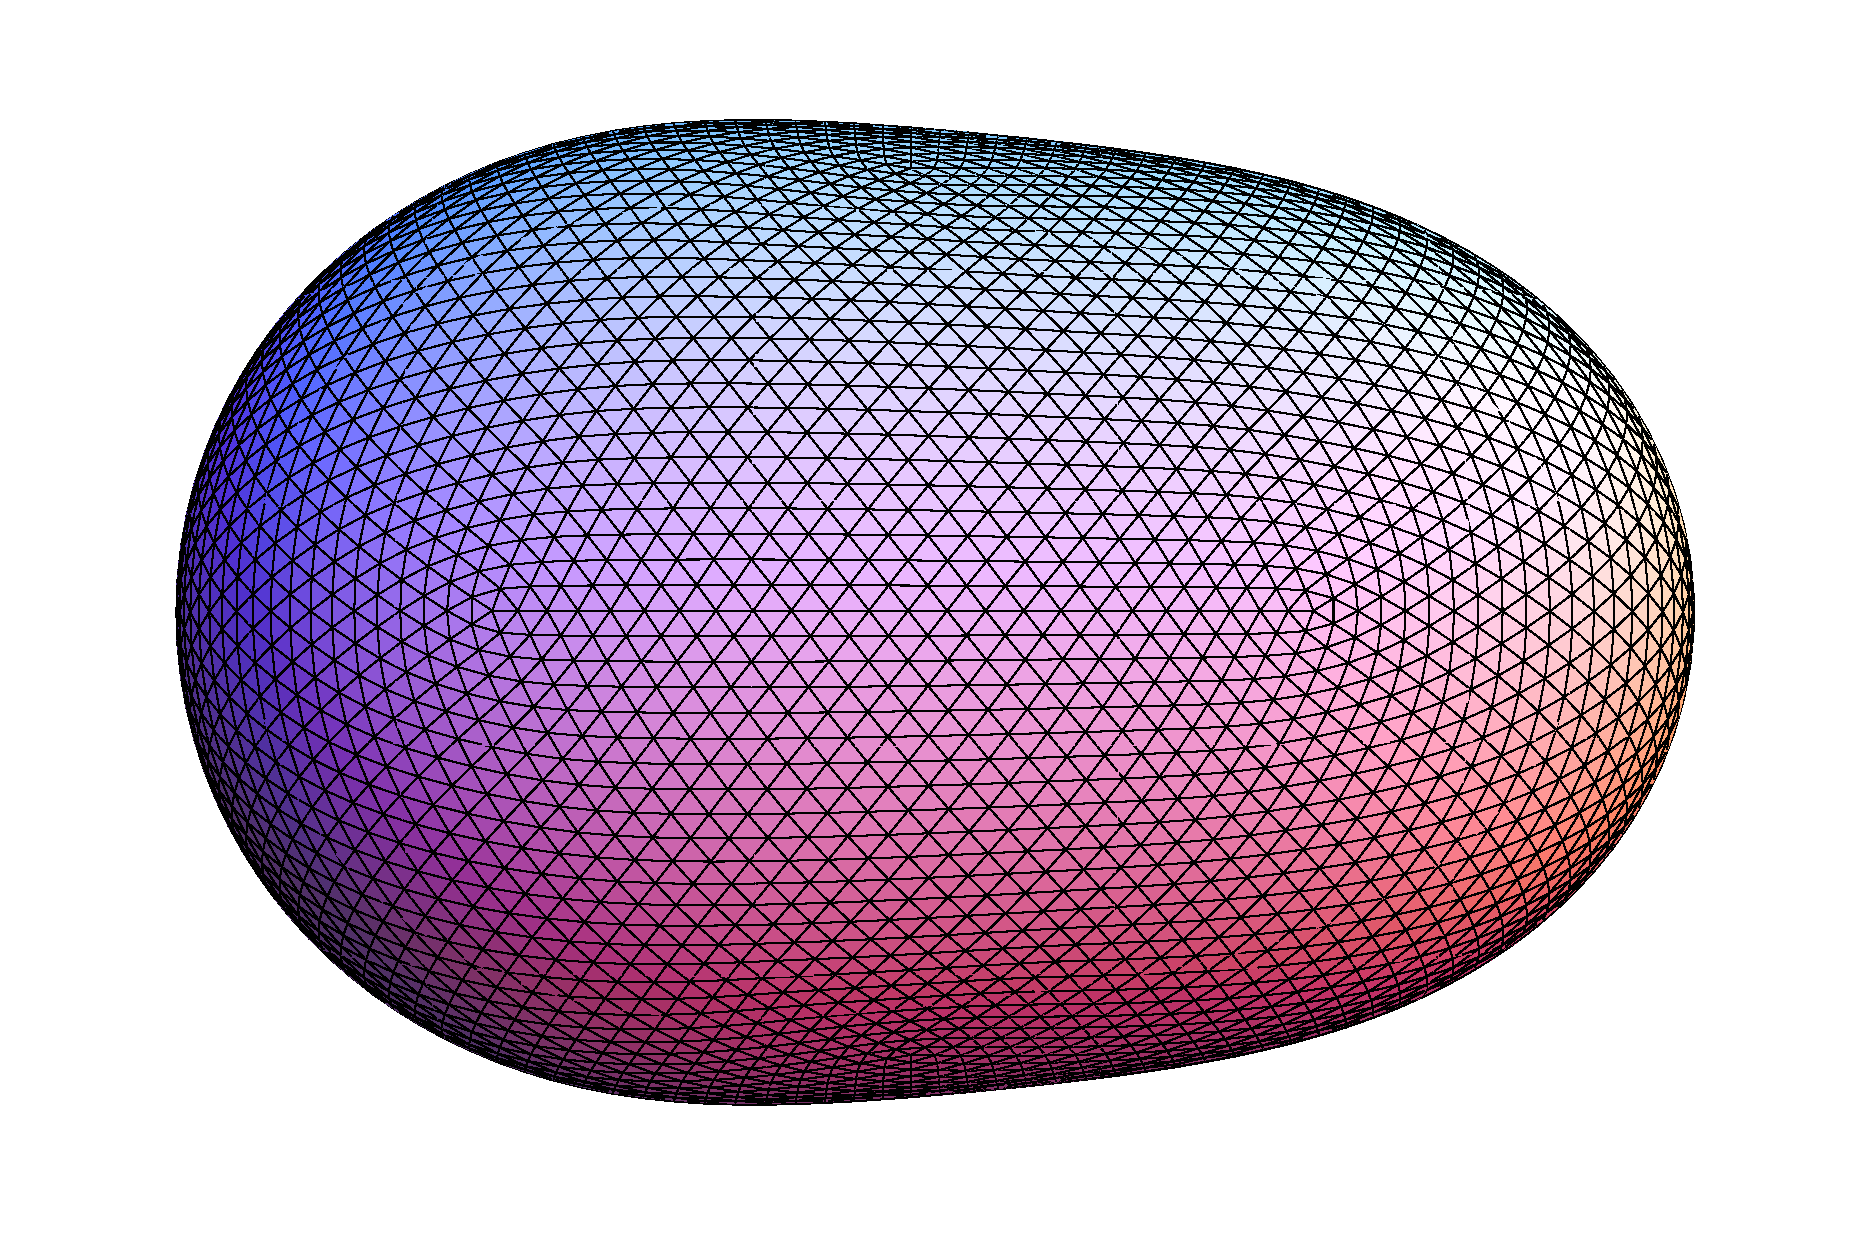
\includegraphics[width=0.4\textwidth]{shape/shape_vred95_conf95_v1eb20}
	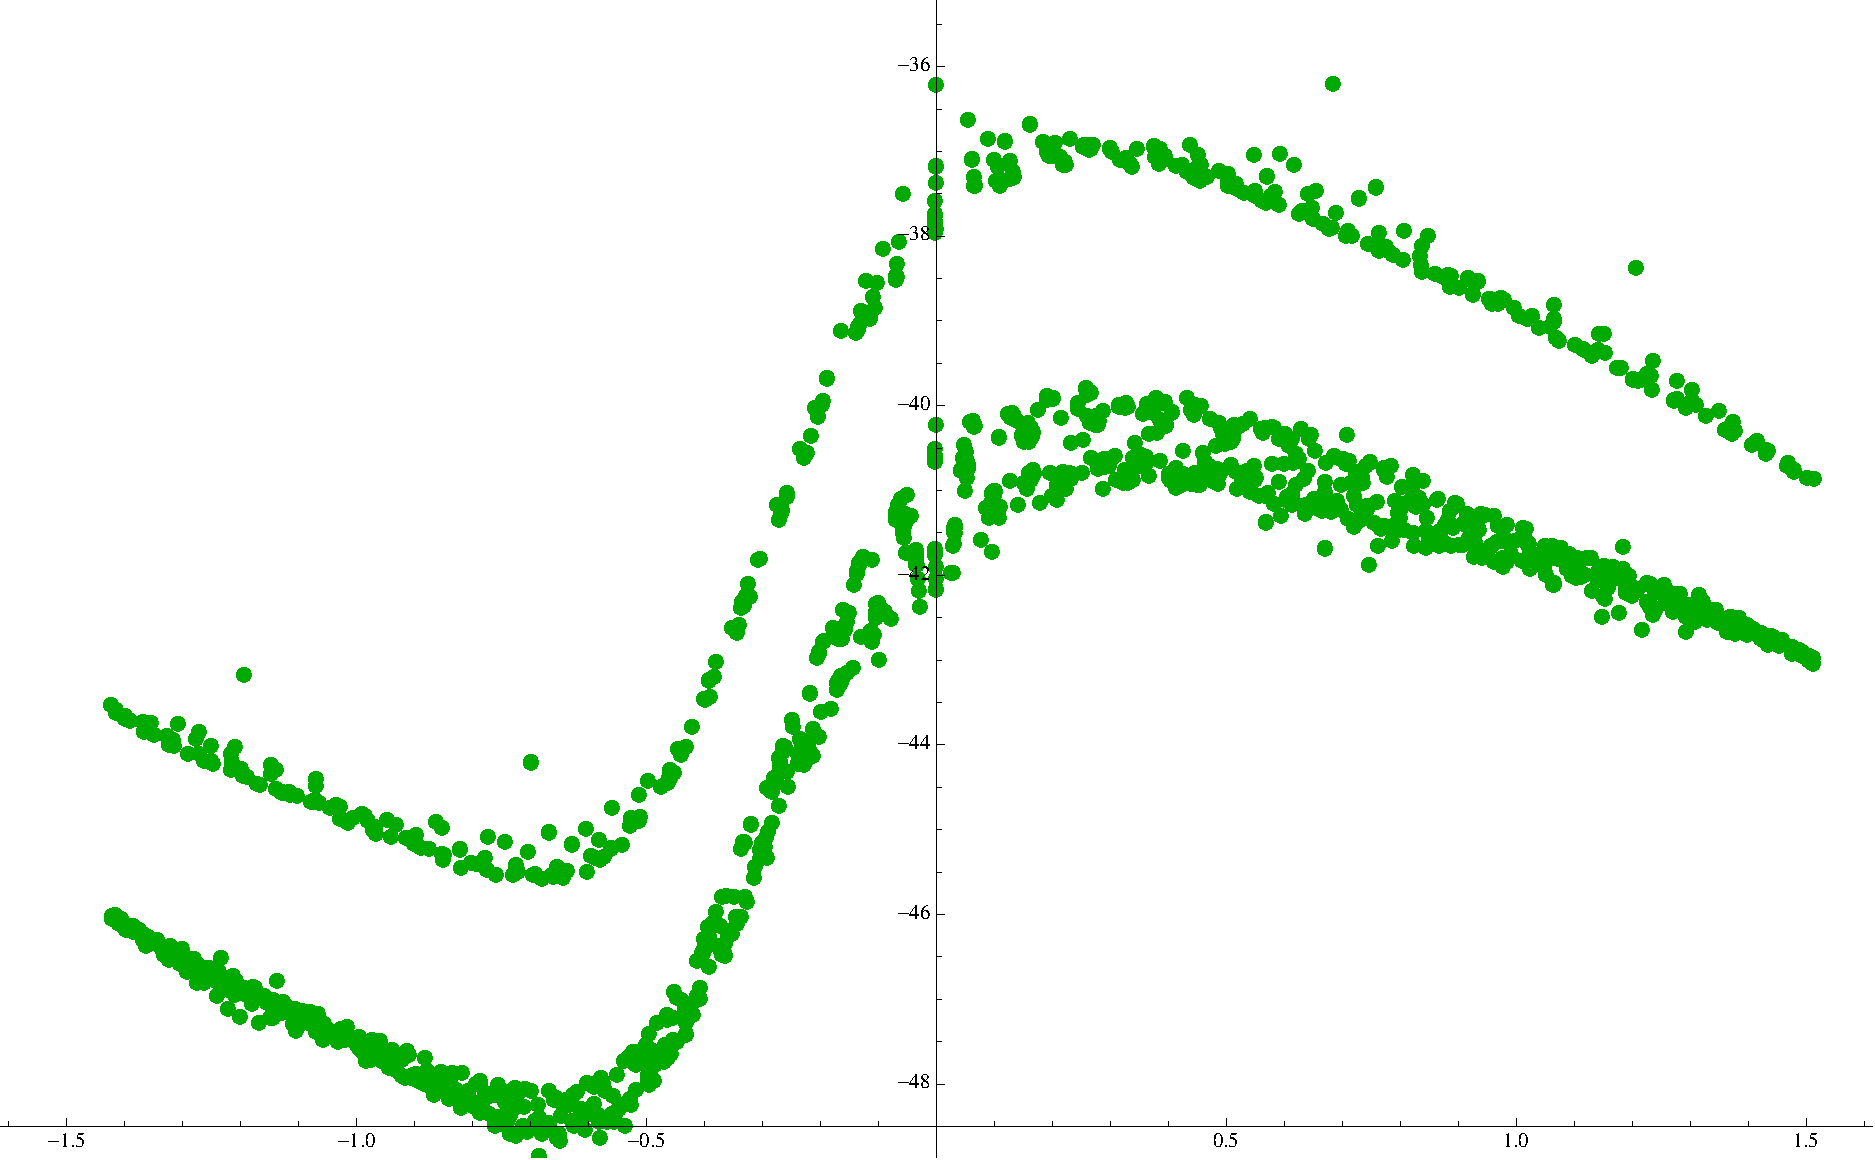
\includegraphics[width=0.4\textwidth]{tension/tension_vred95_conf95_v1eb20}
	\\
	Ca = 0.06
	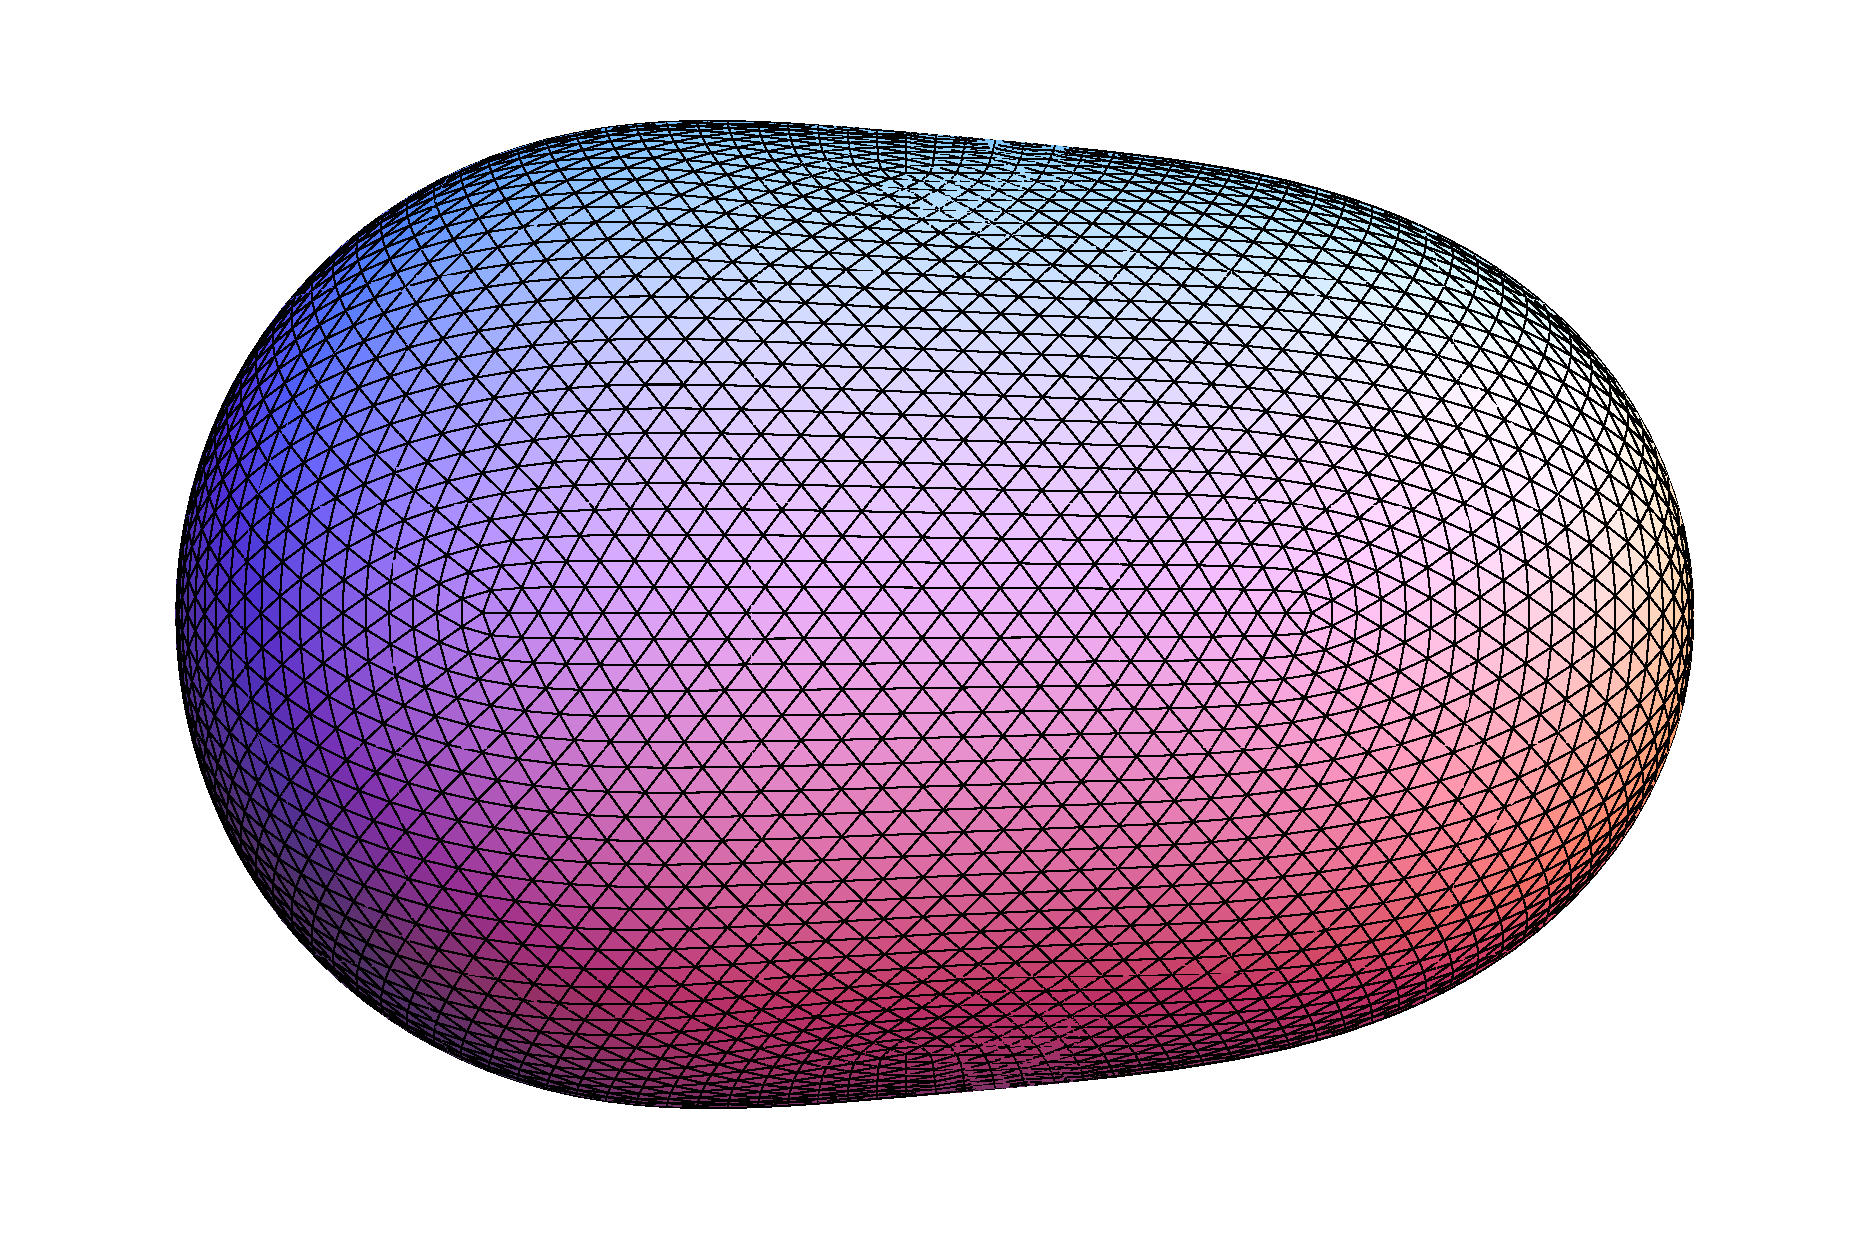
\includegraphics[width=0.4\textwidth]{shape/shape_vred95_conf95_v1eb10}
	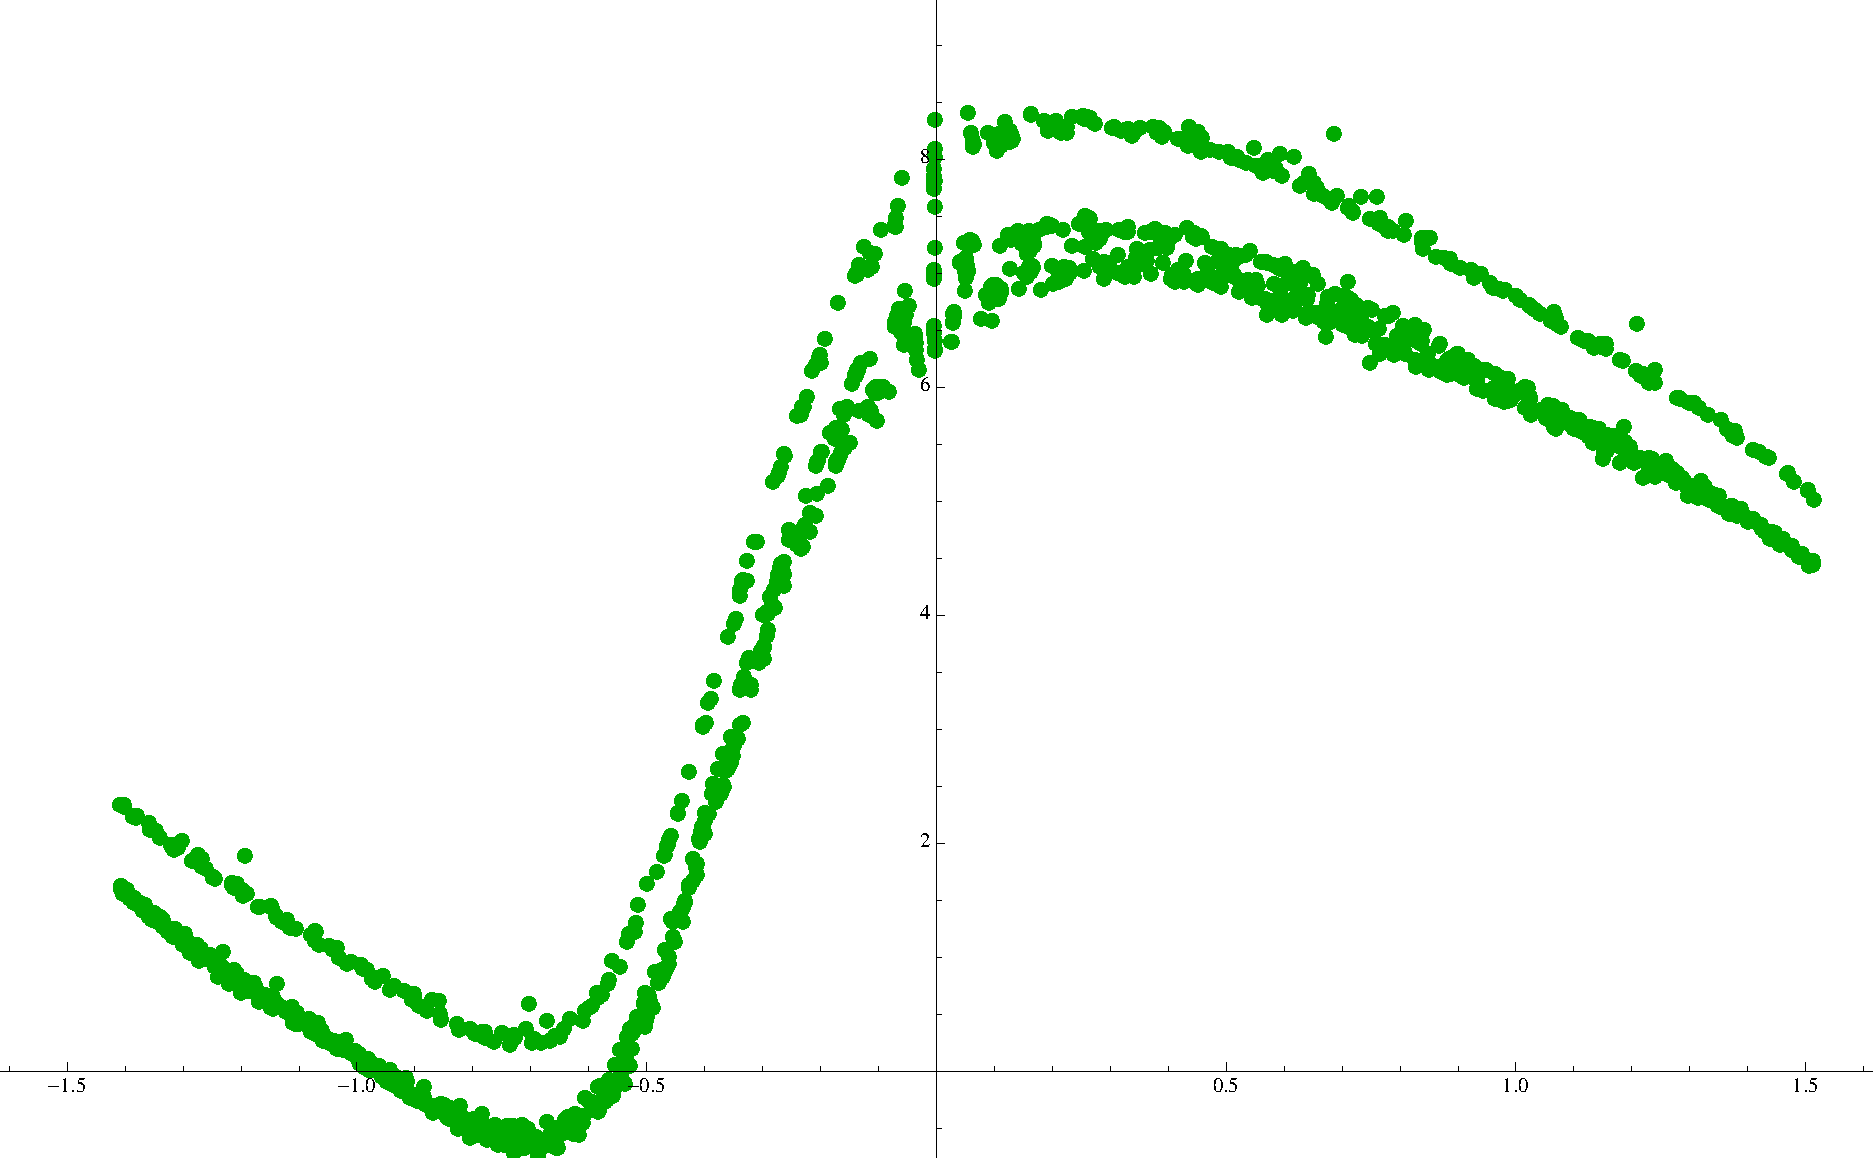
\includegraphics[width=0.4\textwidth]{tension/tension_vred95_conf95_v1eb10}
	\\
	Ca = 0.31
	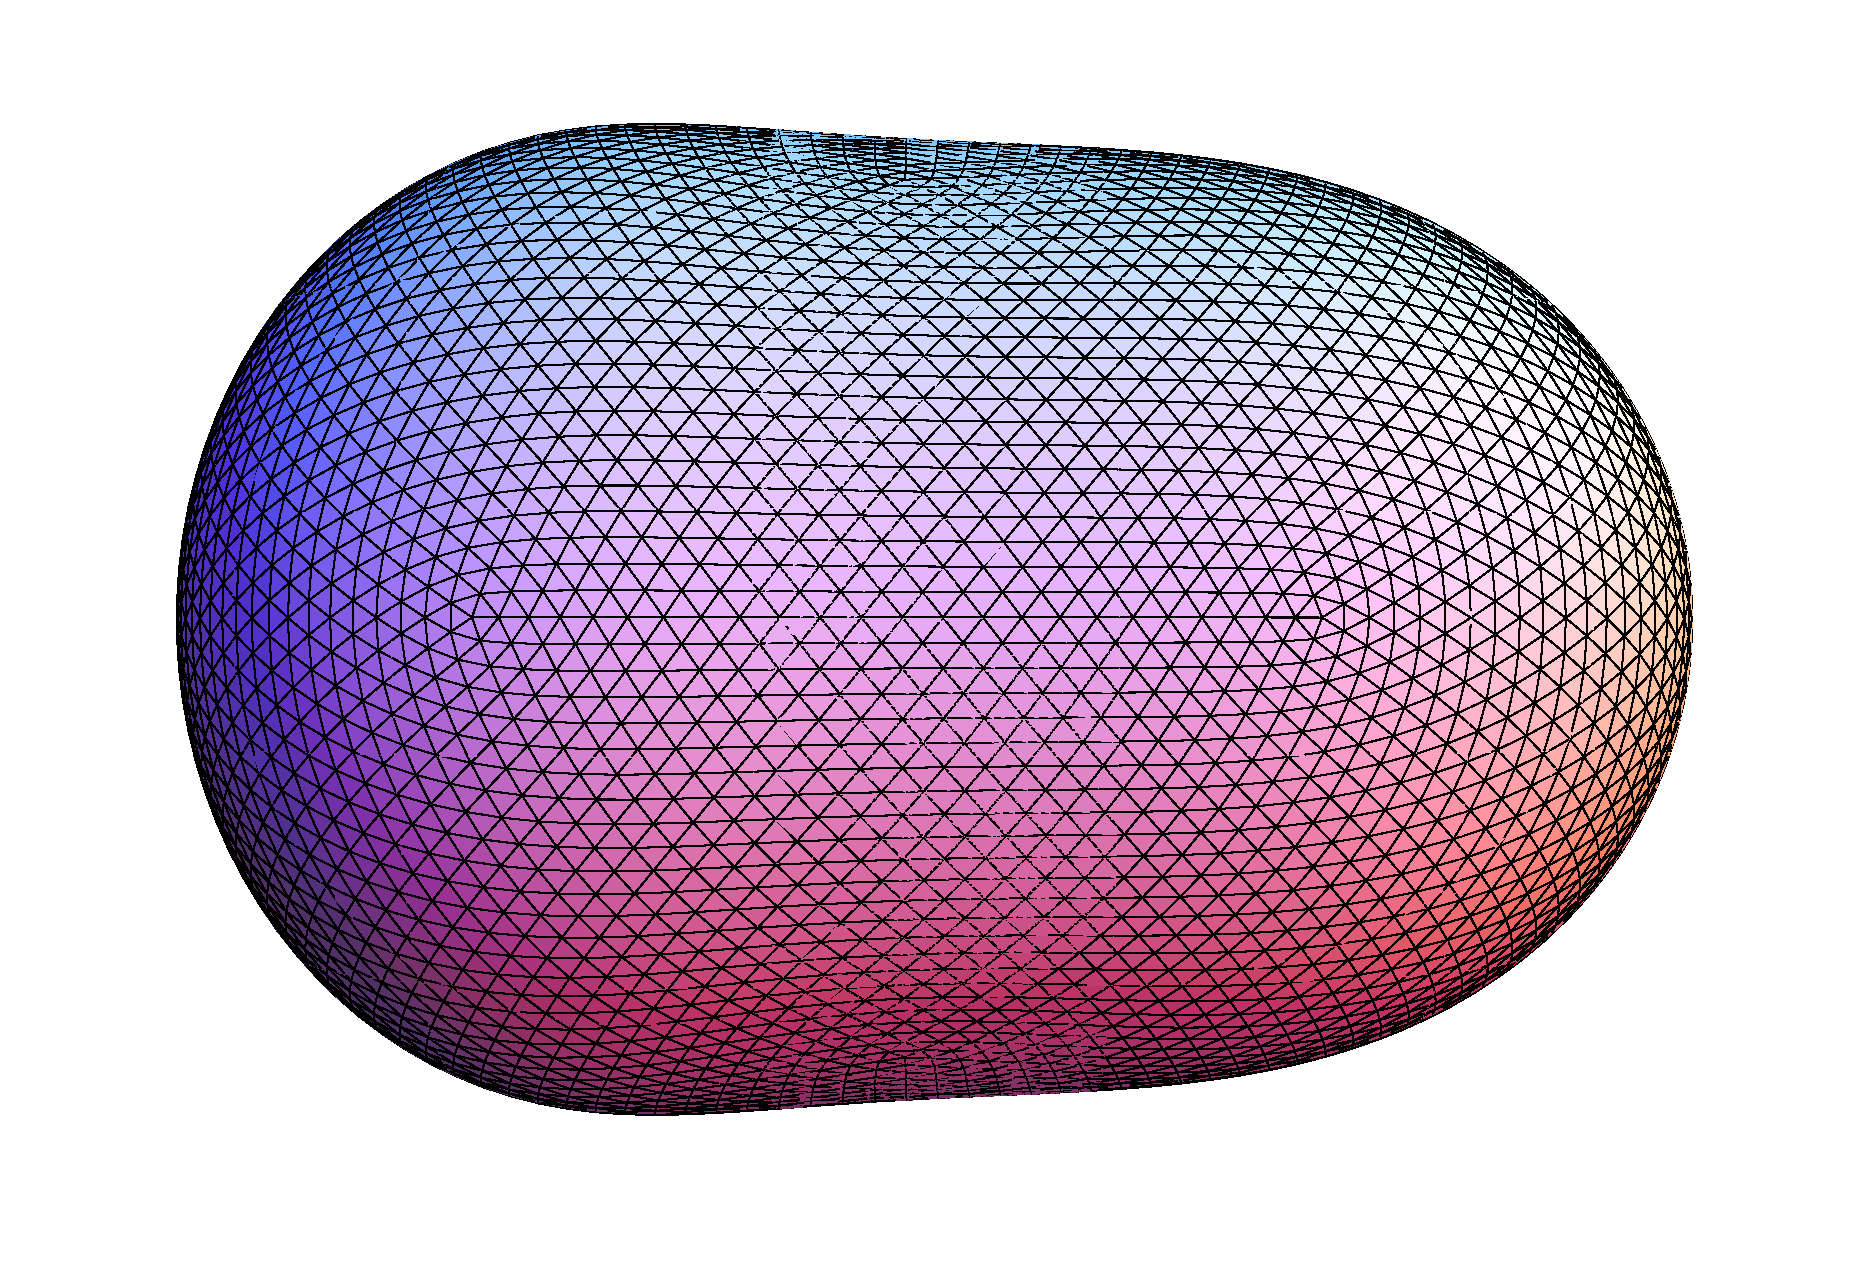
\includegraphics[width=0.4\textwidth]{shape/shape_vred95_conf95_v1eb2}
	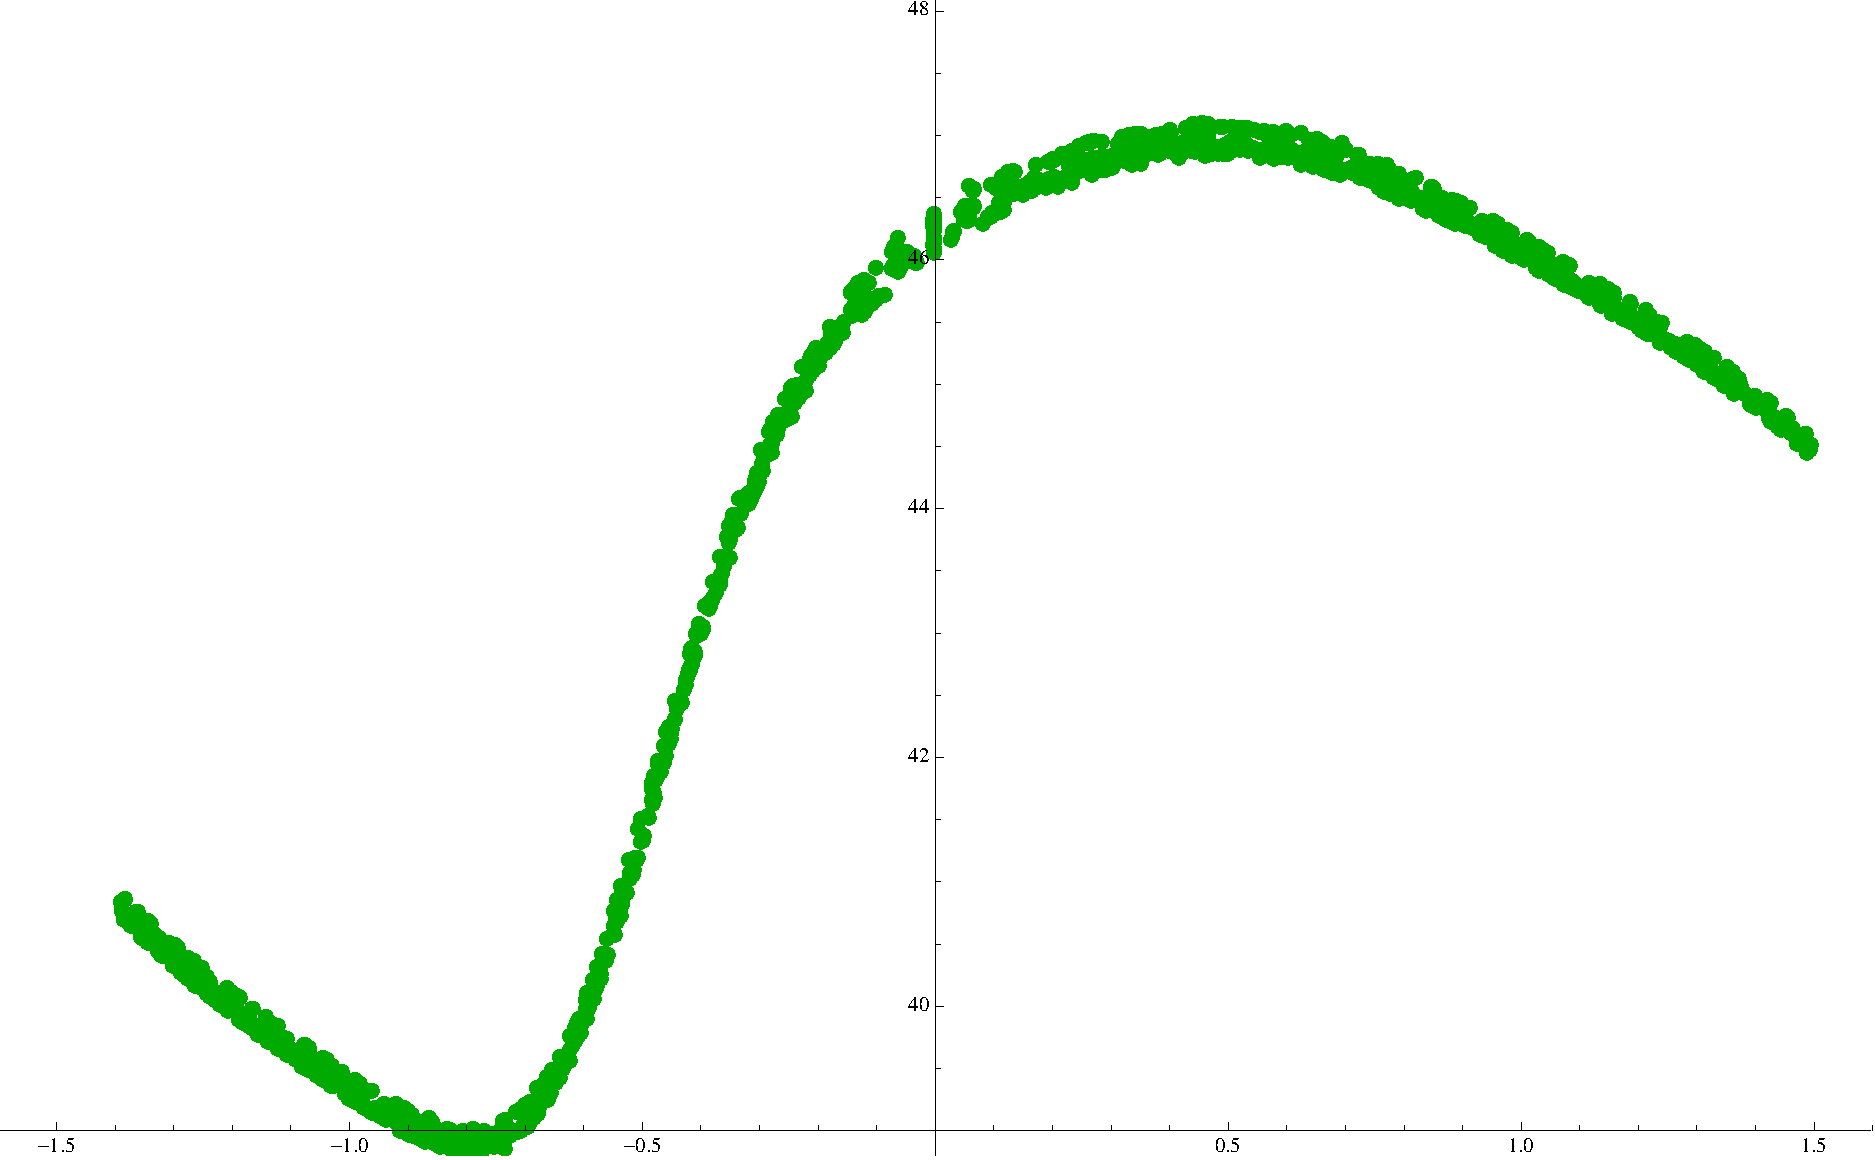
\includegraphics[width=0.4\textwidth]{tension/tension_vred95_conf95_v1eb2}
	\\
	Ca = 1.25 
	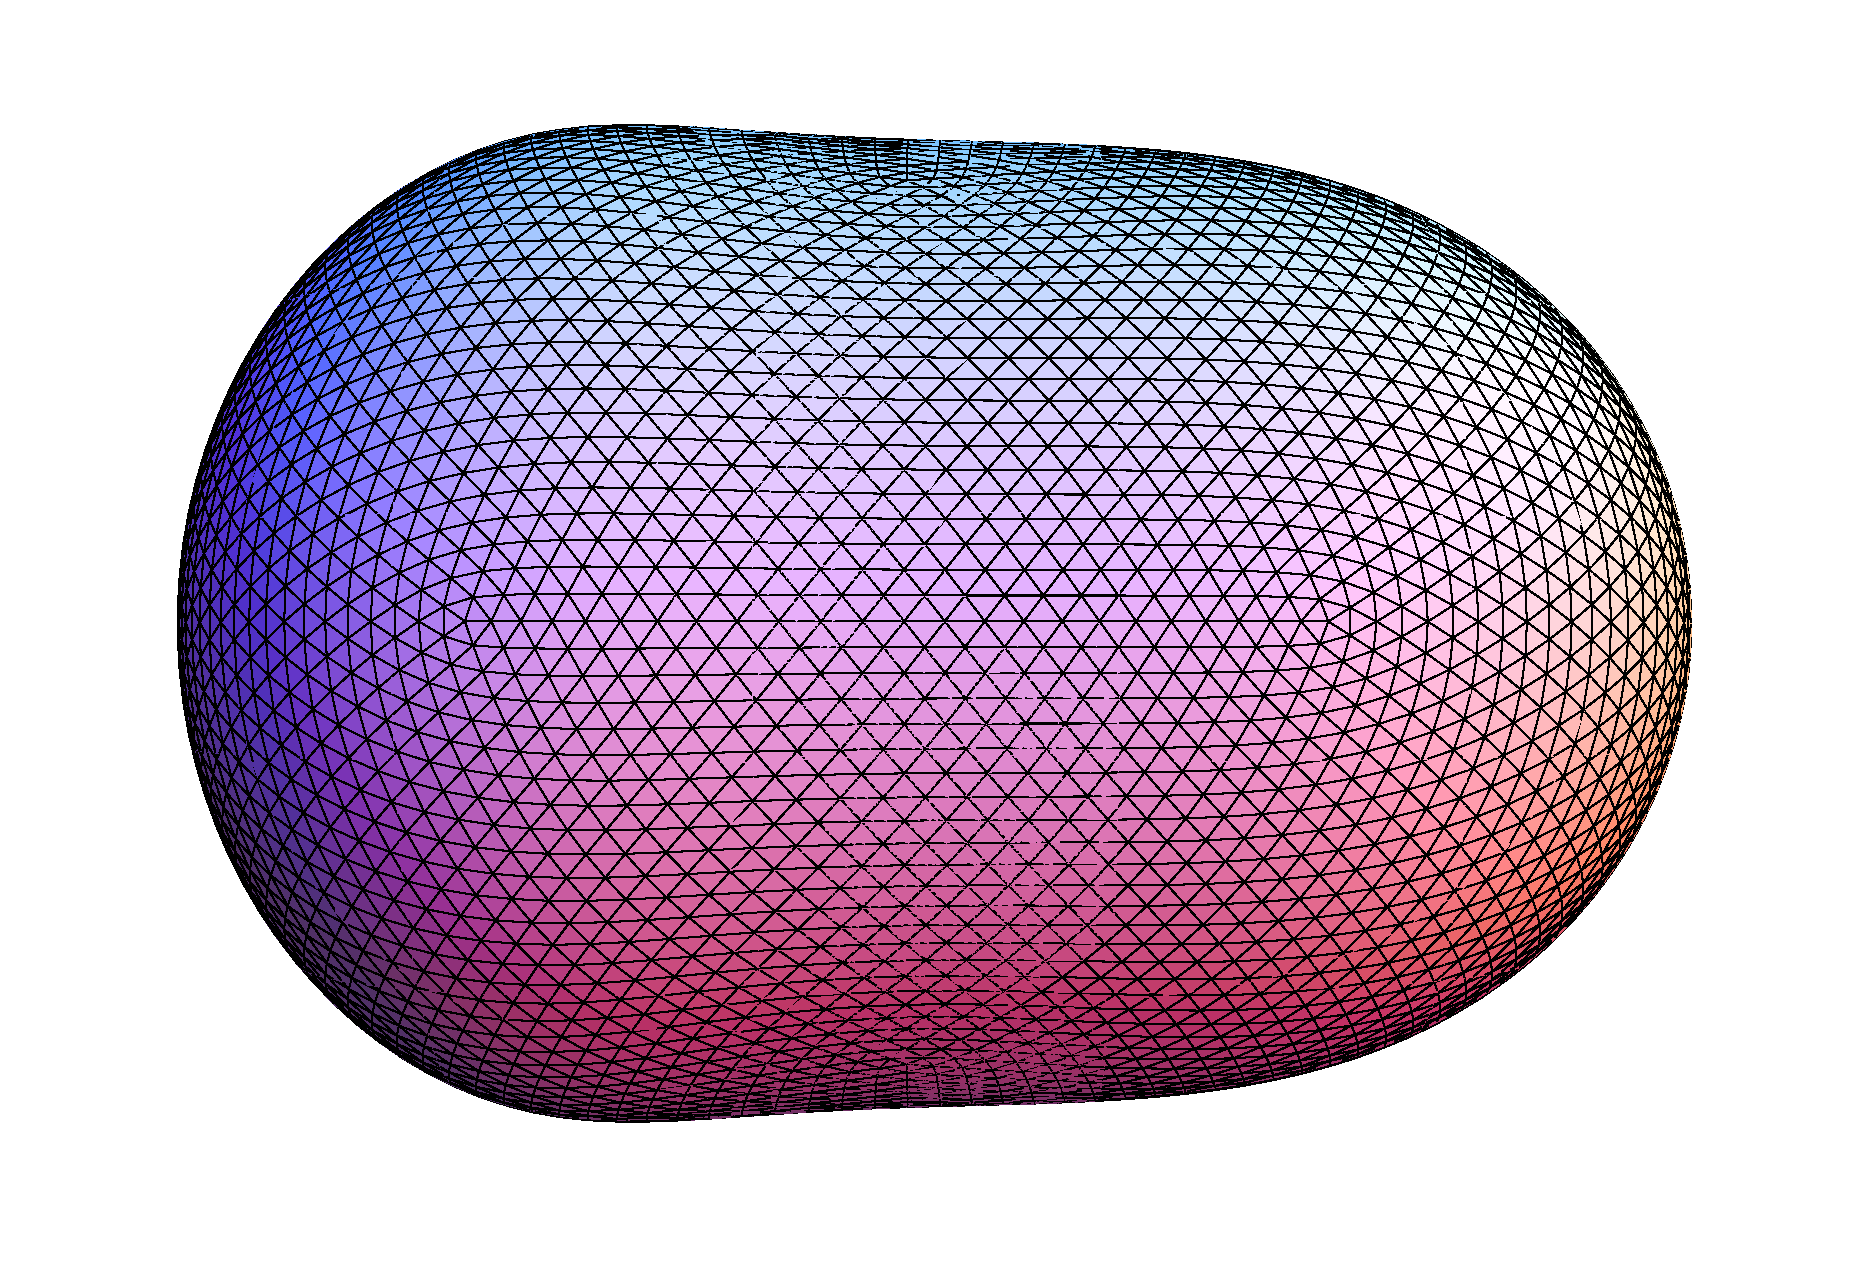
\includegraphics[width=0.4\textwidth]{shape/shape_vred95_conf95_v1eb05}
	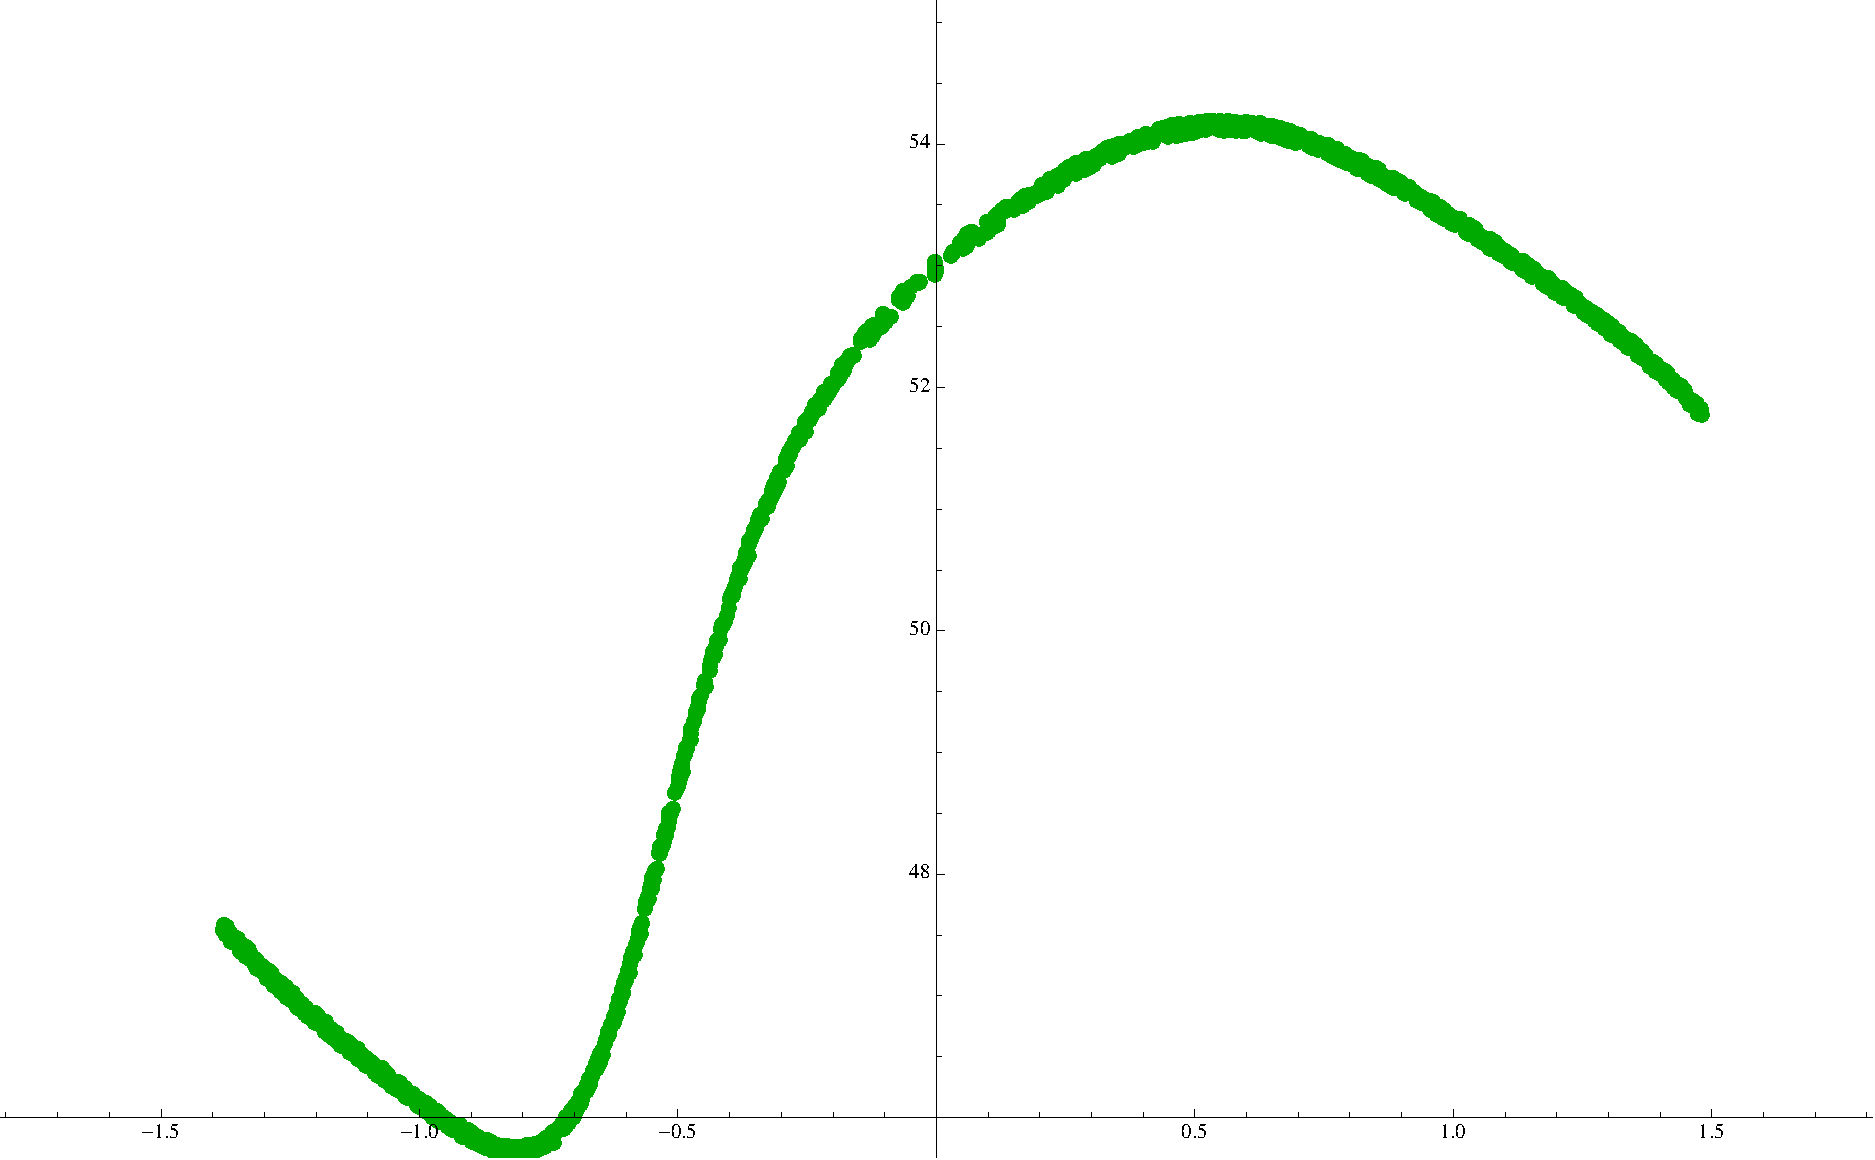
\includegraphics[width=0.4\textwidth]{tension/tension_vred95_conf95_v1eb05}
\caption{$\nu = 0.95$, conf = 0.95}
%\label{default}
\end{center}
\end{figure}






\end{document}